\documentclass{article}
\usepackage[left=2cm, right=2cm, top=1cm]{geometry}
\usepackage[utf8]{inputenc}
\usepackage{amsmath}
\usepackage{enumitem}
\usepackage{float}

\title{Hyperspectral Imaging Biodiversity}
\author{Hannah Gallagher}
\date{October 13th, 2024}

\usepackage{natbib}
\usepackage{graphicx}

\begin{document}

\maketitle

\section{Introduction}

%Convolution 
%Eigenvalues Eigenvectors 
%Discrete fourier transform 
%Continuous transform 
%Vector basis 
%Circulant matrix
%Euler relation



% Hot keys to remember: command / on a mac comments highlighted code in and out.
%Nugget the snowman wishes you good luck on your research!

%\begin{figure}[h!]
%\centering
%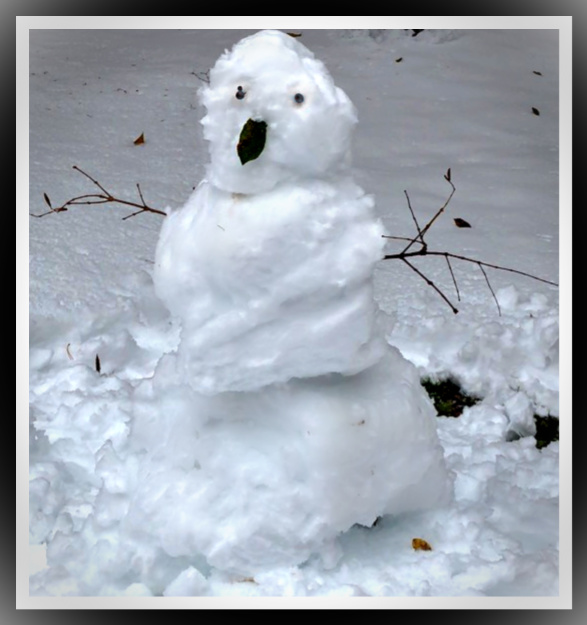
\includegraphics[scale=1]{Nugget.jpg}
%\caption{Nugget the Snowman}
%\label{fig:Nugget}
%\end{figure}

\section{Given Information, Key Terms, and Things to Remember} 
\begin{itemize}
\item Hyperspectral Imaging
\item ENVI
\item Radiance
\item https://scienceandtechnology.jpl.nasa.gov/dr-marc-simard
\item Parameterization of stuff and that NASA problem 7 on pset 2
\item Solid Angle 
\item All the different definitions around radiance, irradiance, radiant intensity etc.
\item 4PIX
\item Edge Detection
\item Global Warming
\item Salt Marshes protect ecosystems
\item LiDAR shows more fine details


% \begin{figure}[h!]
% \centering
% 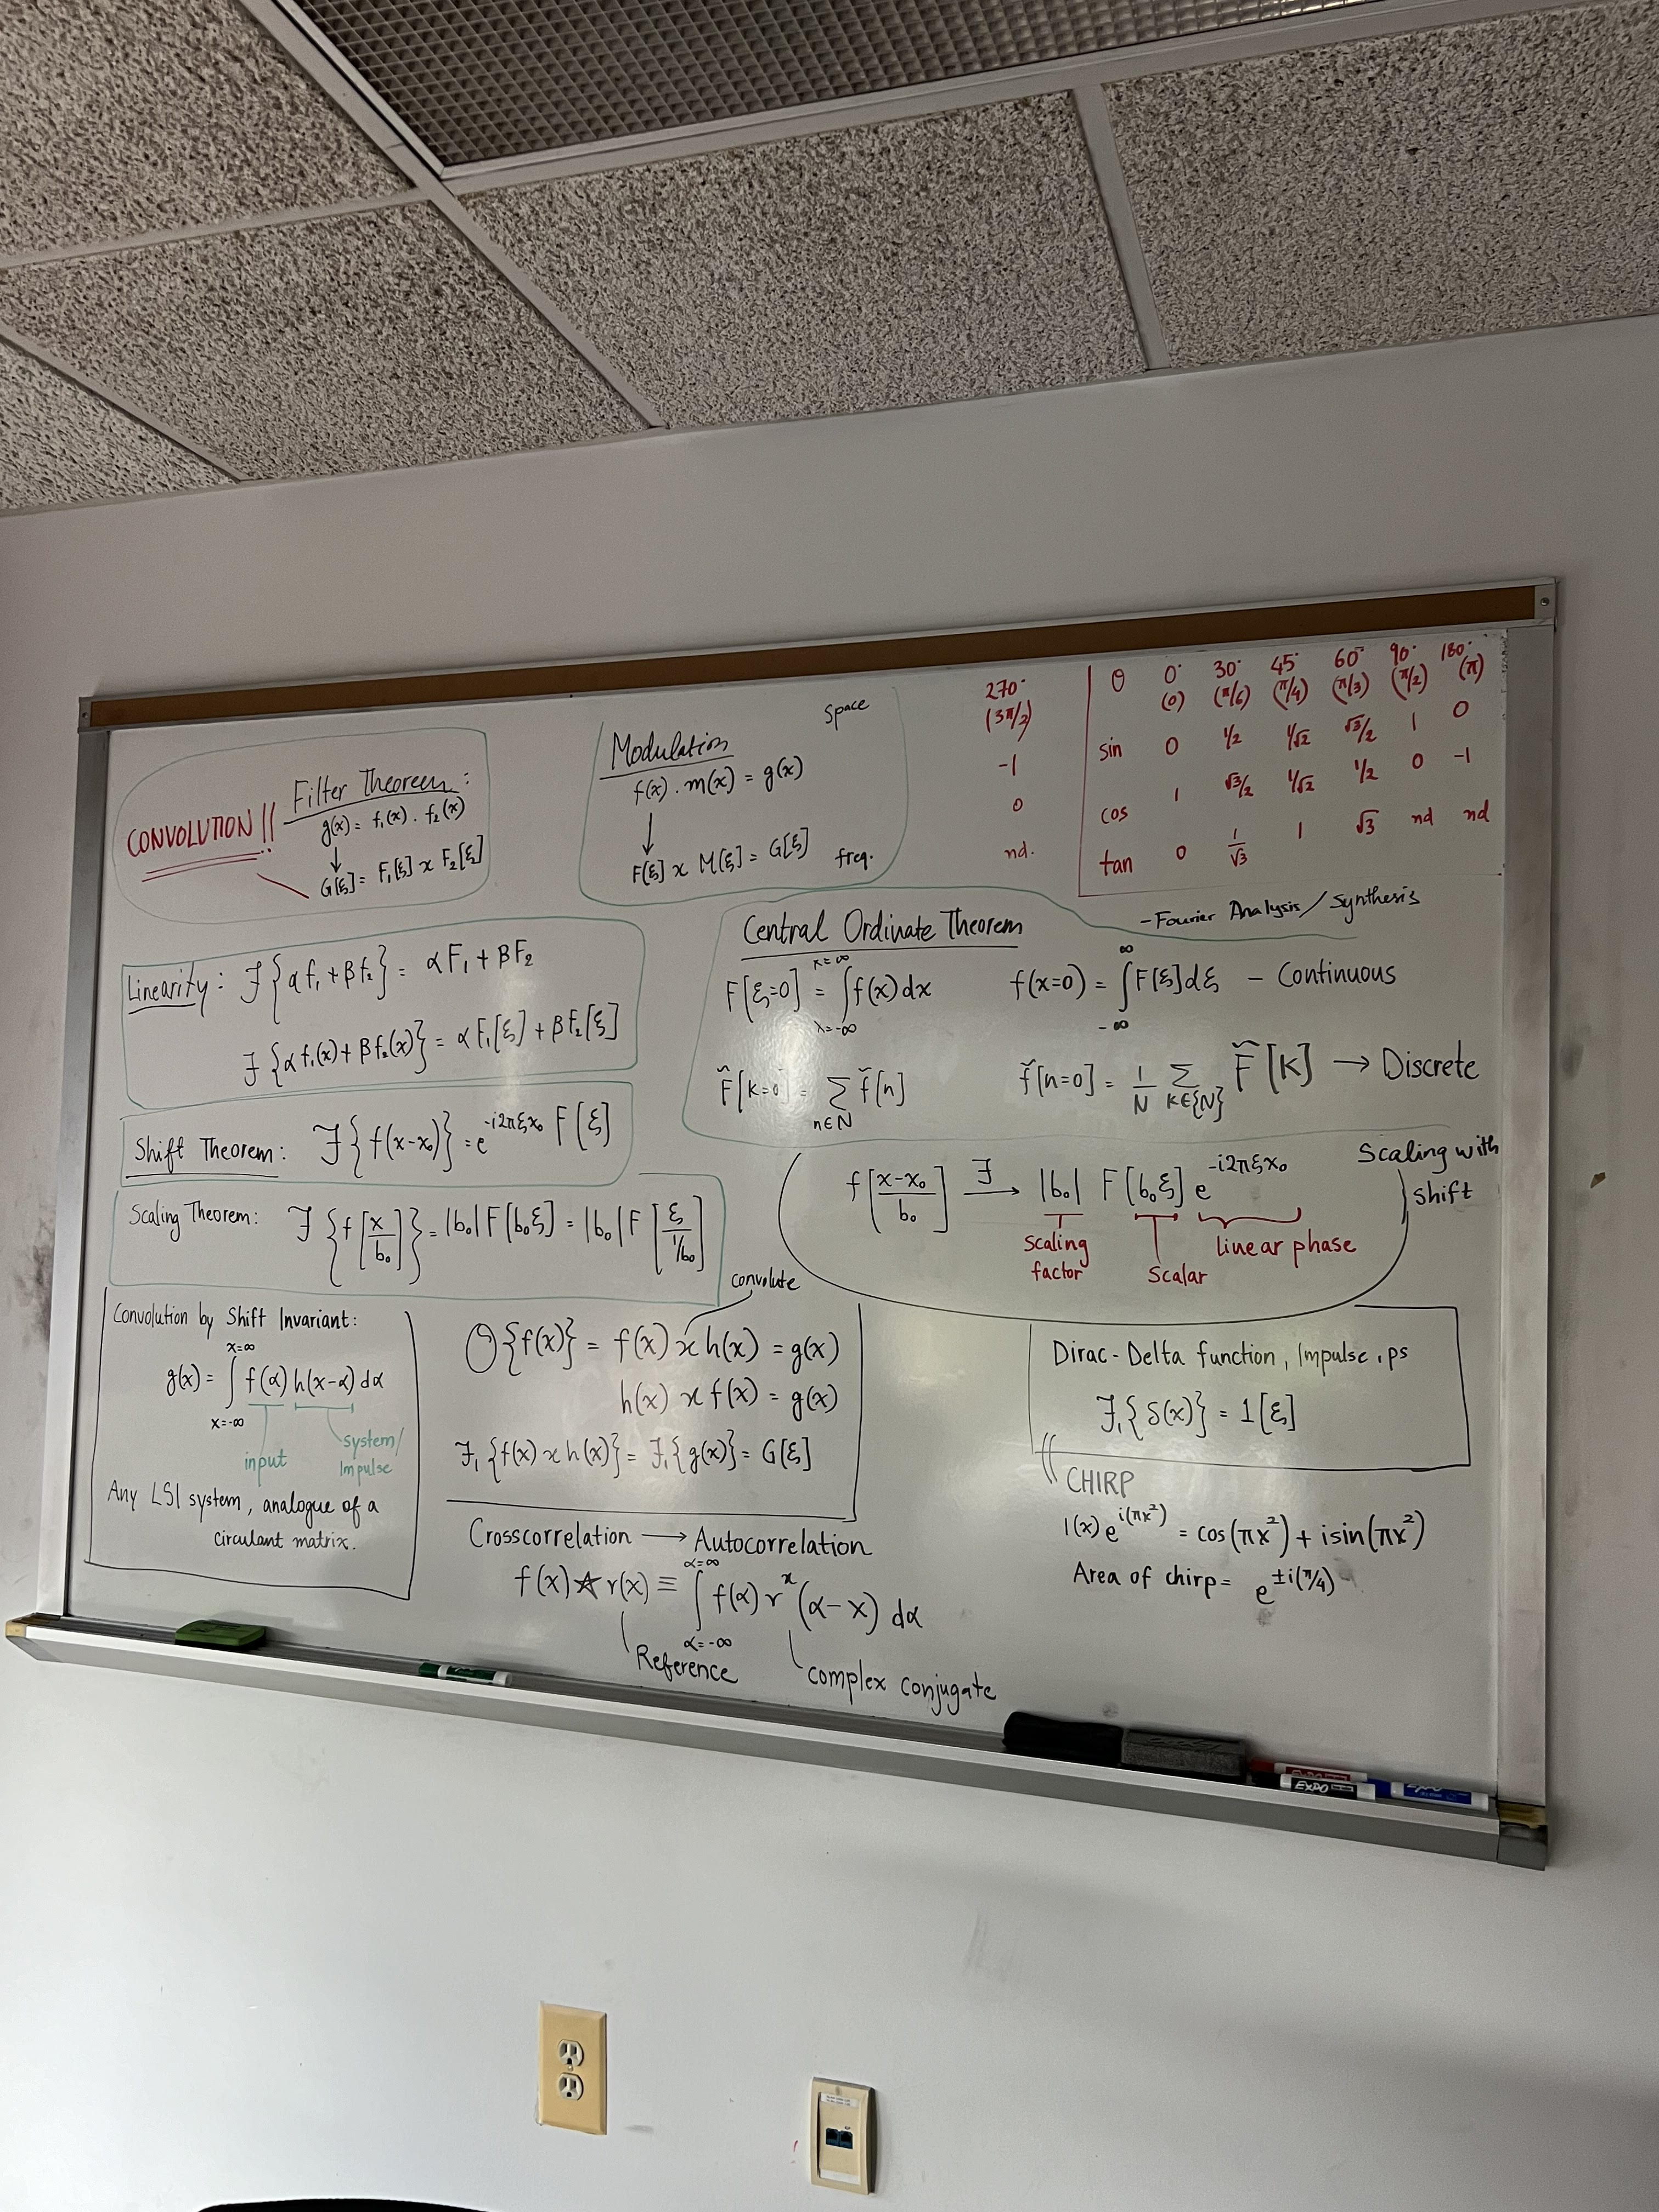
\includegraphics[scale=.20]{Fourier/unnamed.jpg}
% \caption{Easton Syllabus}
% \label{fig:Snowman4}
% \end{figure}


 
\end{itemize}

\clearpage

\section{Day by Day}

\subsection{October, 2024}
(Beginning stages in another document along with weekly GRIT meetings are in a google doc.)
Nayma wrapping up research and explaining how to use the dat files and open shape files in ENVI as they all need to be present to view the file. 

\subsection{November 8th, 2024}
Finally achieved the mosaic image in ENVI during the research meeting. Asked about a hard drive to borrow.



\subsection{November 13th, 2024}
Research meeting after the second Fourier exam. Received the hard drive to borrow as it was okayed to be cleared.

\subsection{November 15th, 2024}
Week frees up a little bit and made plans to read more papers on hyperspectral imaging, red edge, and ENVI over the weekend. Quick check in with Dr. Bachmann to ask about possible meeting times. Grant due Monday for Dr. Bachmann so Tuesday meeting planned. (Will also have to be quick).

\subsection{November 21st, 2024}
Undergraduate research presentation for AWM and PiRIT. Practiced public speaking and speaking about research. 

\subsection{November 22nd, 2024}
Bowling with Pure Physicists.    

\subsection{November 23rd, 2024}
Went to High Acres Nature Area. (HANA) 

Studied how I could learn about tree health in marshes from the ground level as everything I'm working in is too small. Need a broader idea to get started. 

See end of document to see pictures from the tree study. 


\subsection{November 26th, 2024}
Studied and read the Radiometry textbook 2-5 again. 

\subsection{November 27th, 2024}
Had the idea to use the human vision review model to do this lit review. Read a few papers that were review papers, but they really only spoke on different software. Looked over the lab data and that may help in the future knowing those fundamentals. 



\subsection{November 28th, 2024}
Read more papers about software, such as random forest, not very insightful as I have already used random forest in past research. Anything done with machine learning was glossed over.  

\subsection{November 29th, 2024}

(Early Morning) Application of leaf multispectral analyzer in comparison to hyperspectral device to assess the diversity of spectral reflectance indices in wheat genotypes: Sunlight is important in analyzes the health of an ecosystem as it is needed for photosynthesis. 
Plant Senescence Reflectance Index. 

(Noon) Read Radiometry Textbook Chapters 7-10 again on the drive home from Thanksgiving. Various relevance to Radiometry as Photometry is not the focus. 

Crop yields paper and fertilizer levels differences\\
(Evening) 10 year high school reunion. Spoke about research and had a few ideas for research topics more relating to human vision. 
Went to bed early and was too tired to look at anything. 


\subsection{November 30th, 2024}
Spoke about research with neighbors at annual Christmas Tree party. Practice for explaining topics and thoughts. Importance of detection of dry leaves for fires as wind blew the leaves towards the fire. Browsed papers when home about research papers relating to campfire smoke in eyes and detectability in satellite, hyperspectral imaging etc. Thought more about Volcanic atmospheric conditions. 


\subsection{December 1st, 2024}
Spent the early morning watching Radiometry lectures again from the midterm to Thanksgiving. Took notes in LaTeX on what was mentioned and emphasized in each lecture. Looked through the homework again. Found the relevant lecture that mentioned all of the important practice problems for the homework.

Continued to work on the lab. Found relevant lectures pertaining to that. 

Continued  to keep up with Dr. Bachmann Google Scholar notifications. Read those papers and then extrapolated from the related OSA papers in one of the beach studies from 2015. Found a study on the development of white radishes in China which require ample nitrogen which relates to Nayma's work. 

Browsed ENVI's abilities and help menu. Downloaded more photos. 

My dad wanted a marble ball bee water feeder for Christmas and I looked up some papers on how it worked. Apparently bees see in UV light. I already know a lot about bees so that could be an avenue. 

\subsection{December 2nd, 2024}

Early Morning: Read papers on hyperspectral and LiDAR imaging of bee and floral biodiviersity.

QUESTION: 
How can Lauren detect the snails she's studying for their biodiviersity in the marshes? Aren't they too small? They're most likely brown so in a muddy environment they probably blend in. Could she simply be looking for the plants or looking at different pictures that are closer to the ground?

Plan: 
Continue to work on Radiometry Lab and Homework. Do easy questions for Fourier. Submit final draft outline for Human Vision. Listen to more papers while grading etc. 

Tomorrow: Finish up Fourier homework. Work on Lab and ask questions. 

Wednesday: Go to seminar to ask questions and work on Radiometry Lab. 



\subsection{December 4th, 2024}
Group meeting and ask everything I had directly that was in this document. 

\subsection{December 5th, 2024}
Human Vision Final. 


Meeting with Dr. Bachmann. 
\subsection{December 6th,2024}
Radiometry lab cram as there was no other time to do the brunt of the work. Sleep deprivation and stress. 

\subsection{December 7th, 2024}
Recover from the lab. Three hours of sleep and then polish the lab to have better workmanship habits. 

Call it quits in the morning and nap. 

Caaught up on errands and everything pushed because of how busy the week was. Printed out review packet. Decorate tree to de-stress. 
Looked over lectures. Try to stay up, but was still sleep deprived and passed out watching a lecture. 

\subsection{December 8th, 2024}
Tried to memorize practical resolving power equations and grating equation. Paid attention to what was emphasized and not in lectures. 
Watched Radiometry lectures September 10th-November 7th 2024. Made folders and took screenshots of important moments and put them in each lecture day's folder. Worked a little to be able to afford retaking classes if necessary (kept me off my phone). 
Read textbook. Scalded left hand with coffee and went home. 
Wrote out solutions to hw number 1. Was worn out from the pain of the coffee burn so had to listen to old music to feel something and get re-motivated. Realized that I needed to listen to music earlier in the semester because it helped a lot. My original logic was that I would remember what was said in lectures if that was the only thing I listened to, but it probably made life too monotonous despite the lectures actually being fun with the random interjections.  

\subsection{December 9th, 2024}
Went through all the lectures for Radiometry. 
Studied with Muskan, Jason, Triya, and Aisha for Radiometry. 


\subsection{December 10th, 2024}
Studied for Fourier and Radiometry with Tony. We went over optical depth problems. Asked Dr. Easton questions for an hour about Fourier. 

\subsection{December 11th, 2024}
Studying for Radiometry. Wrote out all the homework problems and made a review sheet for everyone. 

\subsection{December 12th, 2024}
Radiometry Final Exam. Forgot about shot noise camera problem even though it was on my study sheet. Met with Dr. Easton later to ask questions for an hour. 

\subsection{December 13th, 2024}
Fourier Final Exam. I don't know what I got, but I remembered all the formulas and had thoughtful answers. I answered practically every problem. Bothered Dr. Easton for last minute questions before the exam. 

\subsection{December 14th, 2024}
Wrote a really good Human Vision review paper in less than a day on Migraines with aura. 


\subsection{December 15th, 2024}

Continued to read the paper that I found where Dr. Bachmann was cited. "The Reflectance of Solar Light from Natural Surfaces." 
Graded papers for Numerical Analysis as I put that off to get through finals which was approved by Dr. Lousto. 

I want to have at least 350 days where I committed to Github (they can be minor changes such as an update) so that no matter what the outcome of the semester is that I still have a plan and am being productive. I know I needed a break last year, but I did not work enough. 

\subsection{December 16th, 2024}
Got up early and finished grading the papers for Numerical Analysis. Caught up on Soleo work and started looking at my winter project...wishing for more hours. Returned to the gym and everyone said, "Hello stranger." 
I had classic talks with people about how I should help find water on Mars or asteroids. 

\subsection{December 17th, 2024}
Reviewed Radiometry slides and lectures (seventh time) for my own benefit. 
Meeting with Jan and Dr. Bachmann. 
Jan meeting went well and I can be a hybrid student. 

\subsection{December 18th, 2024}
Review anything that I missed in Radiometry in the early morning. Start winter project for Soleo. Back to doing more technical analytics now that I have bandwidth. 

Read five papers from the google drive for the research group. Including BRDF and soil moisture content. Hapke model papers seemed empty so I need to find a few on that on my own. 

\subsection{December 19th, 2024}
Focused on Soleo work. Did some QA on Allstate. Started my winter project and produced a spreadsheet for a point to start at for gaining new affiliates. Then I sent this finished spreadsheet to my boss and looked at SEMRush to do some analytics. 

Got Radiometry grade and processed it. Looked through some of the lectures to see where I went wrong. I did better in Fourier and that is objectively harder. Memorizing is clearly not my strong suit. Maybe I spent too much time on blackbody theories. Usually putting too much weight on a class usually has the opposite effect I want as then I am stressed. I'm not sure how it went this wrong though. Maybe the snow threw me off, but that shouldn't be a factor. I made the study document. I studied with people. I made flashcards. I watched the lectures a ton. I redid the homeworks. I highlighted the textbook throughout Thanksgiving break. Most of what was on the exam had something related to it in my study guide. I didn't know much about the coral problem, but I understood the theories. I reviewed the fundamentals in the second and third problem a ton. I probably should have gone in person since reading the problems took too long. 

It was all doable and possible. I am rusty with these fundamentals and being an A student, but undoubtedly I made progress this semester whether my grades reflect that or not. 

Downloaded chapter 2-8 of the Hapke Radiative Transfer textbook to decide if I can handle the material. 

\subsection{December 20th, 2024}
Clicked around to find SEMRush Traffic and referrals csv exports for Soleo. I have been catching up on doing the December calls for Allstate. 

The Elm story of the diseased trees in the 60's from my dad. Need to follow up to see some of these trees in HANA. 

I read through more of the radiative transfer book. I need to decide what other class to take, but they are all good options. It would help to read each book. 

%I had some car trouble today so hopefully it will not be a problem in the future. Good thing I am technically online student so I should be able to make it work if the jeep bites the dust. 

\subsection{December 21st, 2024}
%Ran errands, painted, wrote, attempted to ship present. Visited Grandma. 

Caught up on December's calls for Allstate. 

In BRDF Science Direct Papers Yamaguchi et al. I learned that snow avalanches are caused by "rain falling on snow" which would make the area heavier thus providing a stimulus to an avalanche. 

Emailed Grover for more information about the Optics course. I will have to wait until after the holiday to ask Dr. Messinger. 

%Need to cancel subscriptions. 

Watched youtube lectures on metrology to prepare for interview. 


\subsection{December 22nd, 2024}
Worked a little. Went bird watching in Hamlin and Braddock Bay area. Saw some snow geese...then hundreds of Canada geese. We spent sometime distinguishing between snow buntings and lapland longspurs. 

%Cleaned for the holidays and wrapped presents. 
%Small Holiday party at our place with Justin's friends. 

\subsection{December 23rd, 2024}
Worked on SEMRush. 
Found out that a textbook I've had for four years, that I got out of pure interest and knowing it was a prominent one, is a required textbook for Optics. 

\subsection{December 24th, 2024}
The holiday. %Read for fun. 

\subsection{December 25th, 2024}
The holiday. %Painted. 

\subsection{December 26th, 2024}
Looked at SEMRush. Read more of the optics textbook. 

\subsection{December 27th, 2024}
Read about hyperspectral research of blueberries in a drought. Continued to read the Fourier Optics Textbook (Chapter 3). Reviewed chapters 1-5ish of Radiative Transfer Textbook. 

\subsection{December 28th, 2024}
Read the rest of Chapter 3 and started Chapter 4 of the Goodman textbook. I need to do more reading on LiDAR point clouds...there has been too much focus on hyperspectral and I think I've been neglecting the LiDAR aspect of the project. 


\subsection{December 29th, 2024}
Fraunhofer diffraction in Goodman book. Read through chapter 5-6 of Radiative Transfer Textbook. 

\subsection{December 30th, 2024}
%QA Allstate Calls
Read Radiative Transfer book Chapters 6-7. Look through the Radiometry supplementary textbook before it expires on the 5th. 
%Finished the spreadsheet for SEMRush sites.
%Caught up on sleep. 
\subsection{December 31st, 2024}
Planned out 2025. Rang in the new year! 


\subsection{January 1st, 2025}
Pages read- 40
Radiative Transfer Chapter 6 
Goodman Optics Chapter 3-4 again. 

\subsection{January 2nd, 2025}
Read about coated particles for chapter 6.4 Radiative Transfer.

Chapter 4 Radiative Transfer. 
Chapter 7-8 Radiative Transfer. Reflectivity and Diffusivity. Lambert's Law. I need to review Legendre polynomials. 

\subsubsection{Google Drive Readings}
BRDF and Radiative Transfer Drive ScienceDirect
Read NEO - Evidence for aqueous altered surface - Keywords albedo. Low albedo asteroids. 
Pages read - 85 including Radiative Transfer Textbook.

%Finished calls for the 26th.
%Kind of want to be the top .01 percent of Taylor Swift Fans on Spotify
Asked a friend that knows about Metrology what books they recommended. Picked up some textbooks and some remote sensing books prior to their text. I'll pick up the rest tomorrow. 

Read Chapter 2-3 of the original Hecht optics textbook. Read the two of the Alonso papers before he was in Rochester. 

Total pages read for today - 145 pages
Need to continue the third folder tomorrow in the google drive. 
%Review Matlab and Wafers and semiconductors and tolerancing


\subsection{January 3rd, 2025}
Checked out the recommended metrology textbooks and finally found a book on tolerancing optical elements. 
Read chapter 9 of Radiative Transfer. I don't know what $h_c$ is. Apparently cylindrical coordinates makes it harder to do the SHOE and CBOE thing. 

I do not understand much about Alonso's old papers. Only in a glossary sense. 
Pages read - 35
%Soleo review of calls. 
%Had some brain fog from working so much yesterday. 
\subsection{January 4th, 2025}
Read about tolerancing in Geneseo. Unsure of what they will ask on Tuesday. 
Read up to Chapter 10 of Radiative Transfer textbook. 
Read the Radiative Transfer section of the supplemental textbook for Radiometry. 

Pages read - 103

Learned of the original paper that started it all for Radiative Transfer from 1905 about foggy atmospheres.

Articles read this week- 20
Textbook chapters this week - 6
Articles read this year- 20
Textbook chapters this year - 6
Readings this year - 26

Pages read - 200 %estimated this was also listening to audio articles all day. It was a lot. 

\subsection{January 5th, 2025}
Reading papers for Corning interview. Found papers written by old friends. Went down a rabbit hole. 


\subsection{January 6th, 2025}
Power hour day. Corning interview tomorrow. Found some helpful youtube videos for review and continuing to look for technical journal papers. Revived my bullet journal from the holidays. 
Plan: 
Review Diffraction Gratings. Remember to emphasize geometry. 
Review wafers, semiconductors, and machines. 
Review Matlab, Python, Zemax, and NLP Project. Came up with practice questions for tomorrow. 
Articles read this week - 28
Chapters read this week - 10

Pages read - 100 %estimated

\subsection{January 7th, 2025}
Prepared for corning interview. 
Articles read this week - 32 (one really long paper from 1974 of papers published and talks at an Optics Society of America conference)
Textbook chapters read this year 10 
Articles read this year - 32

Pages read - 73 %estimated

Preparing for the corning interview was 373 pages read in articles plus the textbooks so plus another 130 pages so 503 pages total for the corning interview plus 8 hours of Youtube tutorials. 


\subsection{January 8th, 2025}
Got another corning interview, well phone screen. This internship is actually in corning. Caught up on Soleo work and read a few more of the Alonso and Forbes papers, but was confused by them. 

Pages read - 20

\subsection{January 9th, 2025}
%Caught up on Soleo work. 
Finished the 1974 Optics Society of America Congress paper so another 15 pages. 
Went into campus to pick up the Jackson Electrodynamics textbook from the library. Talked with some people and found a polarization chapter for my phone screen with Corning tomorrow. Reorganized the beginning files of the first half of the semester for Environmental Remote Sensing into my Google Drive. Set up my printer with black ink. Submitted my independent study form for Radiative Transfer. Hopefully my loan processes soon. Renewed my parking permit. Slower day. 

Pages read - 30

\subsection{January 10th, 2025}
Corning Phone Screen Prep. I read 15 pages of the optical lens design book by Warren Smith, but read more articles for 20 pages about GRIN, liquid lens, and optical fibers. The phone screen went fine, but was not as long as the other one. % I need to figure out finances and things if I'm going somewhere for a summer internship. 
%Met with Makensie for disputing calls and did work for that. 


\subsection{January 11th, 2025}
%Caught up with friends from high school and Imaging Science. 
Read Chapter 13 from Radiative Transfer on polarization. - 30 pages. 

\subsection{January 12th, 2025}
Semester starts tomorrow. Moved my big desk to my office area and got printer paper. 
Stayed up last night so technically I read more of the Radiative Transfer Textbook Chapter 14 - 30 ish pages probably. I need to review the lab papers for Jan's class tomorrow. 
%Soleo disputing calls not working. Reviewing Allstate calls.  

\subsection{January 13th, 2025}
Jan's class was interesting and insightful. The lab helped me understand selecting bands and wavelengths in a scatter plot which seems unbelievably useful for research. We then continued to learn about NDVI which also will come in handy over the time that I am writing my thesis. 

%Soleo meeting with Makensie at 3 pm onsite at Soleo.
\subsection{January 14th, 2025}
Read the 3 articles for astronomy in BRDF and Radiative Transfer folder. 22+3+14 pages.


\subsection{January 15th, 2025}
PhD program review committee visited. Apparently I am getting a copy of the MTF textbook from one of them. 

Manuela is speaking at seminar next week on my old general relativity project. I never finished it to its full potential so I wanted to finish reading the papers, but not get too distracted. I learned that MHD also incorporates radiative transfer so that would be useful.

I am and have read this basically some mini book by Jose A Font "Numerical Hydrodynamics and Magnetohydrodynamics in General Relativity." called Living  in Relativity. It's been a great review of what I did. Currently on page 32. I should probably put in easybib each paper i read to keep up with them. 
Font, Jose; A. “Numerical Hydrodynamics and Magnetohydrodynamics in General Relativity - Living Reviews in Relativity.” SpringerLink, Springer International Publishing, 19 Sept. 2008, link.springer.com/article/10.12942/lrr-2008-7. 


Gonio in Goniometer is from the Greek word "angle."

Painter, Thomas H., et al. “Automated Spectro-goniometer: A spherical robot for the field measurement of the directional reflectance of snow.” Review of Scientific Instruments, vol. 74, no. 12, 1 Dec. 2003, pp. 5179–5188, https://doi.org/10.1063/1.1626011. 

I'll give myself 83 pages of paying attention. 

\subsection{January 16th, 2025}
Reread papers on Goniometers. - 40 pages 
Met with Dr. Raqueno to get 4Pix4D set up. 
Got another interview with Corning in Corning for a R and D internship. 
Research meeting where I signed up for getting my name out there in presenting a poster in the grad showcase, getting my proposal project going, presenting on the 30th to our small group, and finding anything to write a paper about. 
Radiative Transfer class told me that the things I learned in the past need to be reviewed, but it's good that I've been exposed to them before. 

The first homework has been released. 
I wrote out all the problem statements ~ 1 hour. 

\subsection{January 17th, 2025}
Reading the last three pages early in the morning after midnight. 

Read 24 pages on the ManTS Goniometer.  

Resubscribed to SPIE and bought my interviewer's article on there. 10 pages for that. 

Read a paper on LiDAR in cars that was open access in SPIE, but I didn't really pay attention so 10 pages for that. 

Took notes on Radiative Transfer starting at 7:30 pm and it is 9:30 now. I took a 30 minute break so 1.5 hours so far. I went over the gradient, Coulomb's law and spherical coordinate review.  

I listened to the textbook narrator, but only kind of paid attention so I'm not going to count it. 


\subsection{January 18th, 2025}
Wrote radiative transfer notes for about an hour...still on flux and spherical coordinates subjects. Going to rewatch some Radiometry lectures. Watched September lectures and need to look at the legendre polynomials from problem set 1 as they may relate problem 5 to Radiative Transfer.

%Soleo work for three hours

%I still need to study for my Corning interview on Thursday. 

20 pages of Corning interview papers. 

Chapter 3-5 for Radiative Transfer. 

\subsection{January 19th, 2025}
3 hours on Radiative Transfer at Starbucks and took notes up to the almost end of Lecture 1. The Laplace equation is apparently important for the homework. 

Fell asleep briefly to papers. 

Saw some short-eared owls. 

\subsection{January 20th, 2025}
Couldn't sleep too much. Found a paper on liquid lenses again about Corning Varioptic. I read this paper a lot, but I kept zoning out. 

I wrote out more notes for three hours or so today. 

%I did my best to do some Soleo work this morning. I sent a report to them in the morning. 

\subsection{January 21st, 2025}
Need to think about my different projects that I can do at the end of the semester and for my proposal. Radiative Transfer class and read Chris Lee's published paper. Wrote notes for another hour and a half. 


Work from home. Read a few Corning papers and asked a worker there about what exactly their sister office does. Had Radiative Transfer today and Chris possibly already has a project so I need to decide soon. We focused a lot on Dipole interactions today. 

\subsection{January 22nd, 2025}
Jan's class today and then Manuela's lecture for seminar. 


Started the morning with S. L. Kandelinskiy and V. V. Tkachenko, "Optical geometric effect of the intersection of matched conicoids as illustrated by line beam scanning," J. Opt. Technol. 90, 563-568 (2023). 


Jan's seminar lecture with some technical difficulties since Emmett is gone this week. Very narrow contiguous bands with hyperspectral images. Look at the silicon range and then they are some vegetation pixel

Plants absorb and then there is photosynthesis. The red edge and inflection point can show vegetation health. Look at water content. Blue is thrown away.  Blue as a green wavelength. LiDAR and emits laser pulses and measures return trip distance. 
D point cloud of a vineyard was shown. Models where the disease is in the beans. See if the canopy is closed up and then look at the point cloud. Facetize the point cloud and calculate normals to each point clouds. Rounded closed canopy and can be at risk to the mold. 

Push broom scanner shown. Whisk broom shown. Flux tower and measures edico changes of the gas flows of a forest and then do predictive models across the whole forest. Then the DIRS lab does LiDAR and then the thermal sensors and then the Nano is silicon wave and SWIR. The Thermal cooled is then quite a lot of money. 12.5 lbs full payload at 120k 1,000 3D laser points m2, 200 spectral color channels then the cheaper version 2 lbs and at 8k and 3d point for each pixel. 5 spectral/ color channels... but the right ones for an application. Then there is a lot done at Cornell and the slow expensive one is uninteresting to farmers, but the faster ones get their attention. 

Cheap drones have broader bands. Wine class. Good red wine and torture the vines to extract the water then they extract the flavor. The vineyeards do a spectral assessment and then the stem water potential. He picks a random set of 30 leaves and in tin foil and then it stops photosynthesis and goes into equilibrium with the state of the leaf and then puts into a pressure chamber and with a gasket and the little stem sticks out and add physical pressure and stop where to see what the plant is pressure is under. 

Leaf level to the canopy level to the drone level. If it does not work at the leaf level then it most likely will not work at the drone level. 
Apple scab and mock infections to look at. 

NEON of the LiDAR and then get a 360 view and then extract the point cloud and then get the structure. Andrea visual shown. Looked at the overlapping geometries. He has funding, but of course not for me because no money for da Hanuh. 

Radiometry and then they validate it to get the imaging science. 



Aaron's research talk: 

DIRS. Landsat technical interchange meeting. Landsat has been launching 1972 before everyone here was born. They have had many satellites. Works with NASA and USGS. Has 11 bands that they acquire data with and then there will be a 26 bands and then how to transmit the data to the ground. Then how much data can be a bad thing. Validation of the thermal projects. Stray-light removal algorithm. DIRSIG Digital Imaging and Remote Sensing Image Generation. Working with the line of sight (LOS). Harvard Forest. Used to test their compression algorithms. Data from Raytheon. 

%Fell asleep after getting my car. Woke up at midnight. 

\subsection{January 23rd, 2025}
Reading papers from Kochan's paper. 
Research meeting. 

Went over Poinying vectors in Radiative Transfer and Maxwell's Equations with magnetic fields and charge density flows. 

Allow for a free current and there is no net charge and charge is free to move in the lattice. Induced current is sigma. 


\subsection{January 24th, 2025}

Met with Dr. Weinstein and I'll go to his recitations on Thursdays at 2 pm. Dr. Raqueno helped me set up some permissions with delta and my password is the password without data. She will be back Friday next week. 


\subsection{January 25th, 2025}
The notes were posted up to the 4th week so I think it's time to buckle down and try to get ahead. I'm optimistic, but I know how these things work out in reality usually. I think I should review the notes by just looking at them as well as writing them out. I wish there were more hours in a day. 

I went to a networking event in the morning and got some value from that and free food. I had a friend take notes on the rest of the meeting as I am too busy now. 

When I got home I did some Soleo work and then took more notes on the second lecture. I took notes for about 6 hours yesterday on Radiative Transfer. 

I read that paper by Asner for EnviRemote yesterday. 

%I've been trying to stay up when I can as it may be harder to do certain things as America falls apart. Hopefully the equal opportunity act being repealed doesn't affect me. It was an hour before my interview...I'm worried I won't get a FASFA for the fall semester so I need to make a lot of money before then. 

\subsection{January 26th, 2025}
I finally got up at 8 am and now I want to get to the third lecture at least today for Radiative Transfer. I got most of that done.


\subsection{January 27th, 2025}
We went over the HSI Asner paper in Jan's class. 
I met with Dr. Raqueno to fix an error I was having. 
I met with Dr. Bachmann for Radiative Transfer. 
%I woke up early so I fell asleep instead of taking notes tonight. 
%I brought in the free food from the Distillery for the 1st year grad students and others.
%I met with Rob to get more done for Affiliate Summitt. 
I feel like I'm falling behind so I need to stay up tonight. 


\subsection{January 28th, 2025}
I did not stay up last night. Radiative Transfer homework extended. 
I went to Dr. Campanelli's endowed professor ceremony. 
7 p.m. 
I read Alonso's paper: 

\textbf{Willow or Alder Shrubs are massive shrubs in Alaska. The U.S. Forest Carbon program does not always count shrubs and leaves the model incomplete. SfM point clouds is a viable option to LiDAR. This also provides RGB data. UAV devices are not properly calibrated to radiometric data though. At the time of the study, LiDAR has not been compared to the "structural measurements" from photogrammetry."Our 
specific objectives were to: 1) Determine the best predictors of tall 
shrub biomass across upper montane and subalpine habitats through 
comparison of SfM point clouds derived from UAV imagery, SfM point 
clouds from NASA Goddard's Lidar, Hyperspectral, and Thermal (G-
LiHT) Airborne Imager, and G-LiHT lidar; 2) Characterize tradeoffs 
among point density, color information, and canopy penetration from 
different point cloud data sources for biomass estimation; and 3) ex-
amine uncertainty propagation through the process of SfM data ac-
quisition, processing, and analysis in a complex vegetated landscape. 
We demonstrate that low-cost, consumer-grade UAV platforms can be 
used to accurately estimate shrub biomass." Adding color to sfm models then it was comparable to LiDAR (for depth?).}

Questions: How do trees absorb water? How is it different in different trees. How do lesions on a tree affect a tree?

\subsection{January 29th, 2025}
Stayed up last night and played with my NOAA radio. I'm going to talk about red edge, hyperspectral, LiDAR, and Sentinel-2 Data tomorrow at the research meeting. 

Power plants have ruined Ireland and left only 18,000 hectares of wetland to thrive. 
Dr. Bachmann's seminar class presentation: 
Roughness is related to bandshape. 

Spectrolon calibration panels for the drones are supposed to be lambertian, but they are not. 

Prosail is a vegetation...thing...I really need background slides for myself and anyone else who finds this useful. 

Do all your work now and this week if you want first dibs on any biodiversity projects. I currently am reading someone's dissertation on marshes in south carolina...if I have time I want to look into how the hurricanes last year affected these marshes. 

\subsection{January 30th, 2025}
Send Optica your resume. 

There is an app called arboreal, which is a tree height smartphone app. 
What is basal area?

\subsection{January 31st, 2025}
I fell behind in keeping up with this. 
I got and accepted my Corning internship job!!!

\subsection{February 1st, 2025}
Journal and publications writing retreat: 
Need to find something that extends the pool of knowledge. 

What contributions does your text in process make, if you have one? 

What are the 'conversations' of your (sub) discipline that you want to join or contribute to? 

I only know about quantum computing in physics. 


Google says:
"Common questions in remote sensing research often focus on data acquisition, analysis, validation, and application, including:
Data quality and pre-processing:
How to effectively correct atmospheric effects on satellite imagery? How to handle data gaps or inconsistencies across different sensors or time periods? 
Feature extraction and classification:
What are the best spectral indices or algorithms to identify specific land cover types (e.g., vegetation, urban areas, water bodies) from remote sensing data? 
Temporal analysis:
How to monitor changes in land cover or environmental parameters over time using time series remote sensing data? 
Spatial scale considerations:
How to integrate data from multiple spatial resolutions (e.g., high-resolution imagery with coarser resolution satellite data) for a comprehensive analysis? 
Ground truth validation:
What are the most effective methods for collecting ground truth data to validate the accuracy of remote sensing classifications? 
Application-specific questions:
Environmental monitoring: How to use remote sensing to track deforestation, air pollution, or ocean health? 
Disaster management: How can remote sensing data be used to assess damage from natural disasters like floods or earthquakes? 
Agriculture: How to monitor crop health and yield using remote sensing data? 
Urban planning: How to analyze urban growth patterns and land use changes with remote sensing imagery? 
Sensor technology advancements:
What are the potential applications of emerging remote sensing technologies like LiDAR, hyperspectral imaging, or Synthetic Aperture Radar (SAR)? 
Data accessibility and sharing:
How to ensure open access to remote sensing data and develop standards for data sharing? "

How do you identify these conversations? 


IF YOU CAN: ASK SOMEONE TO LET YOU READ THEIR GRANT. (Obviously keep it confidential.)


It might cost less to publish now rather than later since I'm a student. 

An editor will come in with a vision statement for the journal and they have it in their editorial of what their vision is for the field and journal. 

Want to be on an editorial board rather than a peer reviewer...but it seems bureaucratic. 

Might want to cite what they editors have written to be on the right track of being in the same topic. 

Single blind vs. double blind review. 

Reviewer knows the author, the author does not know the reviewer. Neither is known for double blind review. 


Journal alerts. Quarterly email. 
Query email to the journal editor. 

Research Rabbit. 
Guest editors want the issue to be good so they might help you. Special issues get cited more. Emotion is a big topic right now in this topic. 

Literacy brokers: people who can support the production of your texts in various ways. 


Advisor/ mentor 
collaborators, co-author, tech 
students, labmates, colleagues in program, curator, librarian, industry collaborators, writing center, expressive comm. center - presenting, slides at RIT. 
Journal gatekeeps
editors or translators

People...

Pick your battles. 

Can lose your job if you are not the sole author of your work and then you get this devalued. 

What questions do you still have about academic publishing? 

Where might you find the answers? 

Who might you collaborate with today to keep your momentum? 
Sydney from Christie Tyler's group. 


\subsection{February 2nd, 2025}
Finally finished W2L1 for Radiative Transfer. Two hours of studying Radiative Transfer. Read a paper on CO2 emissions and power plants in the U.S. relating to pulling out of the Paris agreement. What is Prisma? 

20 pages read today - articles
18+12 = 30 for Radiative Transfer textbook Chapters 2 and 3. 

\subsection{February 3rd, 2025}
Jan's class: Homework 2 is on spectral mixing and is a similar concept to Asner's paper. Class let out earlier due to a fire in the science building. 

\subsection{February 4th, 2025}
Woke up at 4 and worked on Radiative Transfer until class. 
Going over the J charge density thing with the J dot. 

Wants to comment on what this actually means: 
Slide 59 or 58. This is really the vector identity we are trying to take advantage of. If you take the dot product of these then you get the J dot parallel. Left with the J part that is perpendicular. The perpendicular component is what matters that is the direction where the field is strong. 

Talking about d omega and Fields of Moving Charges slides. 


\subsection{February 5th, 2025}
I stayed up and found some papers on how America can skew their emissions data and other research papers from NOAA. 

We also went over the Kokaly and Clark paper in Environmental Remote Sensing. I stayed up to read through more Radiative Transfer notes.

I have only read the first three or so. Something about Volkswagen fudging their emissions and fish farming from a NOAA report. 

 U.S. Emissions, NOAA, and Environmental Monitoring
Biber, Eric. The Problem of Environmental Monitoring. University of Colorado Law Review, 2011.

Hare, J.A., K.H. Ford, and S. Godfrey-McKee. NOAA Fisheries and BOEM Federal Survey Mitigation Strategy. NOAA Technical Memorandum, 2022.

Speth, R.L., S.D. Eastham, and S.R.H. Barrett. Impact of the Volkswagen Emissions Control Defeat Device on U.S. Public Health. Environmental Research Letters, 2015.

Evers, D.C., C.T. Driscoll, and M. Cohen. MercNet: A National Monitoring Network to Assess Mercury Emissions in the U.S. Environmental Toxicology and Chemistry, 2011.

Wiedinmyer, C., and J.C. Neff. Estimates of CO₂ from Fires in the U.S.: Implications for Carbon Management. Carbon Balance and Management, 2007.

Stowell, J.D., Y. Kim, Y. Gao, J.S. Fu, and H.H. Chang. The Impact of Climate Change and Emissions Control on Future Ozone Levels. Environment International, 2017.

Engel-Cox, J.A., and R.M. Hoff. Science-Policy Data Compact: Use of Environmental Monitoring Data for Air Quality Policy. Journal of Environmental Science, 2005.

Karion, A., C. Sweeney, and G. Pétron. Methane Emissions Estimate from Airborne Measurements Over a Western U.S. Natural Gas Field. Geophysical Research Letters, 2013.

Pozzer, A., M.G. Schultz, and D. Helmig. Impact of U.S. Oil & Natural Gas Emission Increases on Surface Ozone. Environmental Science & Technology, 2020.

Russell, A.R., L.C. Valin, and R.C. Cohen. Trends in OMI NO₂ Observations Over the U.S.: Effects of Emission Control Technology and Economic Recession. Atmospheric Chemistry and Physics, 2021.

�� Large-Scale Agriculture, Emissions, and Soil Degradation
An, D. Explainable Artificial Intelligence IoT for Smart Soil Carbon Management. ProQuest, 2024.

Maurya, M.J., and M. Vivek. Deforestation: Causes, Consequences, and Possible Solutions. Idealistic Journal of Advanced Research in Physical Sciences, 2025.

Heindorf, C., S. Schüler, and T. Plieninger. Poetic Inquiry to Explore the Relational Values of a Transforming Peat Landscape. People and Nature, 2024.

Khalil, M.I., and A. Walkiewicz. Managed Forestry’s Contribution to Climate Change Mitigation. Frontiers in Forests and Global Change, 2024.

Tripathi, A., S. Yadav, Nishtha, and M. Nkengnamai. Bamboo as a Carbon-Reducing Agricultural Alternative. Springer, 2024.

Feng, Y., N. Muhanmaitijiang, J. Ye, and H. Chen. Microbial Optimization for Sustainable Soil Carbon Sequestration. Frontiers in Microbiology, 2024.

Jatav, H.S., V.D. Rajput, T. Minkina, and E.D. Van Hullebusch. Agroforestry for Restoring and Improving Soil Health. Springer, 2024.


\subsubsection{Seminar with Senior Graduate Students}
Have a GitHub Repo...already have that. Asking about what is in your Git Repo. 

I read a paper on Co2 emissions with wildfires and agriculture before this. Then I read through the Fresnel Equations from Radiative Transfer and did not get the extrapolation. 

\subsection{February 6th, 2025}
Woke up late and by that I mean 4 a.m. I read some papers and looked over ENVI and need to do more with that before I meet with Jan. I want to ask him how to properly save files and what's the difference between all these file formats. Then also what is a temporal analysis. 

I figured out the beginning of some of the Radiative Transfer questions. 


\subsection{February 7th, 2025}
%Deciding on living situation for the summer. 

I spent a lot of time in meetings for GRITT and then we lost power briefly. I need to select points for Nina and she sent me a map of these grid points in basic editior of 4Pix. That will take sometime and I need to do that over the weekend. 

I did not realize I was so far behind on my homeworks...oh wait jk there was an error in ENVI so it got extended.

I spent a lot of time trying to figure out that error in ENVI. 

\subsection{February 8th, 2025}
%Did some Soleo work. 
I started the morning in a relaxed way reading research papers on Polarization and I found a master review from Harvard and Apple. I read the first section/ chapter. 
Looked at Radiative Transfer notes more, but I need to do it in a focused way. 
I secured free eggs from my farm friend and talked about predicting apple yield from the flowers through drone imagery. She agreed that the disease process is not advanced enough to actually be useful yet.

Saw some physics people from so's department. 

\subsection{February 9th, 2025}
It really seems that there are not enough hours in the day. 

I reviewed my ideas for the Radiative Transfer homework, but am not convinced of a few. I need to fix that. 

I got stuck on ENVI classic using the ROI tool. I'll probably need to go in, but most likely later due to staying up late. 
%Soleo busy work and watched the third week of Radiative Transfer lecture.
I spent most of the day scrolling through the Radiative Transfer notes gaining some knowledge and familiarity.


\subsection{February 10th, 2025}
Stayed up working on Radiative Transfer and went to campus all day to work on ENVI. 

\subsection{February 11th, 2025}
Caught up on work work and sleep. I need to write my report the rest of the week and read any papers. 
%I feel now is the time to cut back on work hours already. 

%I stocked up on coffee. 

\subsection{February 12th, 2025}
Need to develop a literature review of what is out there on my research topic this year to be good. 

\subsection{February 13th, 2025}
Gave a research update on LiDAR and what I have been doing in ENVI Remote class. Radiative Transfer we went over the slab model. 
Stayed up very late and wrote my Environmental Remote Sensing Report. 
%I found my lost coffee mug. 

\subsection{February 14th, 2025}
Edited my report. 
%Packed and drove to Ithaca. Renewed my love of nature. 

\subsection{February 15th, 2025}
Read papers on Marmit - 24 pages. (2 reads through one paper and then 1 read from the other). 

Read the first part of the introduction of "Light Scattering and Nanoscale Surface Roughness" (12 pages).

\subsection{February 16th, 2025}
%On vacation 
I read some of the Hapke textbook chapter 4-5.

\subsection{February 17th, 2025}

Change Detection for Remote sensing. 
I read some more of the Hapke textbook 5-8. 

\subsection{February 18th, 2025}
Zoom Radiative Transfer. 

I read the proposals and tried to understand the language and actions that one would take for this process. 

I read some of the Week 6 and Week 7 papers for Jan's class. 
There still is a lot I want to do. 
%The cold winter this week is taking a toll on me. I keep saying I'll stay up...I need to figure this out. 

\subsection{February 19th, 2025}
%Ran a 5k
%Told more people about my internship. Set up apartment application. 

I read chapters 7-8 minus the last half of 8 for lecture tomorrow of the Radiative Transfer textbook.
%Caught up on Soleo work. Keeping debt at bay. 


\subsection{Ferbuary 20th, 2025}
Gave a quick research update as it was undergrad capstone update week. 
Radiative Transfer I ran my Pix4D work so then I could do more tomorrow. 
I did a lot with ground control points. 


\subsection{February 21st, 2025}

Wrote this and need to edit this: I should get credit for working today since I forgot to submit something to github. 


Abstract:
So much of the electromagnetic spectrum cannot be seen by the naked eye, but it contains a vast expanse of information to help interpret the viability of our world. Hyperspectral imaging helps harness relevant bands such as the near-infrared, infrared, and short-wave infrared to access the biodiversity of forests, and in this case, a marsh off the Virginia coast named Hog Island. Along with this, we employ LiDAR (Light Detection and Ranging) 3D mappings and remote sensing techniques. 
With so much land to cover, UAS (Unmanned Aircraft Systems) are flown over the island with multiple tools, including an image spectroscopy sensor and LiDAR camera. In this age, there is more data available than researchers have time to process and analyze. In this study, we seek to expand our model to include the LiDAR drone imagery of Hog Island. 



Methods: 
Using the aforementioned UAS, the marsh is scanned in determined flight paths to produce imagery that can be analyzed in the software ENVI, which is produced by L3Harris. To process the hyperspectral images, ENVI is used to analyze conglomerate images from the drones called mosaics. Through ENVI, environmental indices such as: Leaf Area Index (LAI), Red Edge Detection, and NDVI can be produced and give insights into the health of the marsh. On the LiDAR side we use a software called Pix4DMapper, which was a branch off of EPFL. Checkered black and white calibration panels were laid across the island to tune to the reflectance and radiance data of the marsh later in Pix4DMapper. The data being looked at in these methods were from July of 2019 while later that year in October, mast imagery was taken and will be analyzed to compare and contrast healthy trees at the peak of summer with trees that have reached the end of the yearly cycle. 


Value:

With less park rangers and volunteers available, we have a lot more land to cover to be monitoring the health of our lands. Drone imagery can aid researchers to access the land with the full electromagnetic spectrum (is this true or are we just looking at a chunk? Do we have x-ray cameras on drones?) to understand how climate change and human interference destroys the ecosystems and biodiversity in these lands. The predictive models of combining the already known hyperspectral imagery models with LiDAR gives a detailed picture of the 3D landscape alongside the spectral information. This will aid researchers in distinguishing between different species of trees and animals along with various ground truth data collected at the time of the experiment to do a temporal analysis of these lands. This awareness of dying or migrating flora and fauna can improve the maintaining and protection of other similar ecosystems.


I also met with Tony doing some calibration experiments with GRITT and was on campus a while for a Friday. I usually study by myself on Fridays. 

\subsection{February 22nd, 2025}
Watched lectures for dipoles and read two papers about change detection, but did not understand all of it. 

\subsection{February 23rd, 2025}
Watched lectures on dipole moments, the slab model, and the H function a little bit. I scanned through the lectures and the homework. I hope to review all the slides tonight.

\subsection{February 24th, 2025}
I'm losing steam to actually write things in this that are actually helpful. I've sent a draft to Dr. Bachmann for the grad showcase. 

Read chapter 3-7 and 11 and 14 from Radiative Transfer textbook. 

Watched February lectures on Radiative Transfer. 
%Went for a short run. 

\subsection{February 25th, 2025}
I was trying to get through the Radiative Transfer Hapke textbook again to get a bird's eye view again with knowledge I know now. I stopped paying attention at Chapter 6, but I got to Chapter 7. 

Got up to the end of Chapter 10 before lecture. 
Going over the hemispherical assumptions. 

\subsection{February 26th, 2025}
Submitted edited abstract for graduate showcase. 

\subsection{February 27th, 2025}
Gave research update. 

\subsection{February 28th, 2025}
Slowly working on change detection lab. 

\subsection{March 1st, 2025}
Reviewed supplementary material for both classes. Slowly working as I have been going for a while without a proper weekend. I may regret this pace tomorrow, but the break is needed in the long run. I found something relating to PCA for Jan's class in one of the longer readings that I went through before. I still need to figure out what that dielectric problem means. 



%Scaling back on Soleo work to make sure school is the priority March and April. Reconnecting with New Year's Resolutions. 
\subsection{March 8th, 2025}
I missed a week of updates due to mixing dates for Jan's class. I am sick of my computer and all the privacy and security plus storage problems. I just want to turn them all off. I need to contact Nayma Nur. 


\subsection{March 10th, 2025}
I want 100 papers to read this week. I may not get there, but even 80 would be amazing. 

NUMBER 1 
[HTML] Mapping the surface properties of the Asal-Ghoubbet rift by massive inversion of the Hapke model on Pleiades multiangular images
DT Nguyen, S Jacquemoud, A Lucas, S Douté… - Remote Sensing of …, 2025
A massive inversion of the Hapke model is carried out over the Asal-Ghoubbet rift
(Republic of Djibouti) using high-resolution multiangular Pleiades images. This is the
first time that such an inversion is performed on Earth over an entire image, previous
studies having focused on planetary surfaces. This work addresses challenges such
as atmospheric and geometrical corrections of these images to produce parameter
maps. The use of fast Bayesian inversion significantly reduces computation times …

\subsection{March 11th, 2025}
NUMBER 2 - Red edge
Read a paper on costal red edge. 

Watched the first two or three lectures again for Radiative Transfer. 

%Had to help my parents' at the house so that took sometime now I can finally finish the Radiative Transfer homework. 

\subsection{March 12th, 2025}
NUMBER 3 - Red edge
Morgan, G.R.; Wang, C.; Morris, J.T. RGB Indices and Canopy Height Modelling for Mapping Tidal Marsh Biomass from a Small Unmanned Aerial System. Remote Sens. 2021, 13, 3406. https://doi.org/10.3390/rs13173406

\subsection{March 13th, 2025}
Number 4 - Red edge
Number 5 - Red edge 
Number 6 - Chapter 3 
Number 7 - Chapter 4 
Number 8 - Chapter 5

% \[
%     V= \frac{4}{3} \pi (b^3 + c^3 + f^3)    
% \]


% \[
%     V= \frac{4}{3} \pi (2^3 + 1.75^3 + 1^3)    
% \]

% \[
%     V= \frac{4}{3} \pi (8 + 5.359375 + 1)    
% \]

% \[
%     V= \frac{4}{3} \pi (8 + 5.359375 + 1)    
% \]

% \[
%     V= 19.1458333 \pi \; ft^3  
% \]



% \section{Question 3}        


% From before, 
% \[
%     V= \frac{4}{3} \pi (r^3)  
% \]

% Let C (t)= Volume of the center sphere at time t. 

% At t= 8 min. 


% \[
%     C = \frac{4}{3} \pi ((.75+.25(t-7))^3)  
% \]

% \[
%     \frac{dC}{dt}= \frac{4}{3} \pi ((.75+ \frac{8-7}{4})^2)\frac{dt}{dt} * (\frac{3}{4}) 
% \]
% \[
%     \frac{dC}{dt}= \pi ((.75+ \frac{t}{4})^2)
% \]

% \[
%     \frac{dC}{dt}= 4\pi (r(t))^2 * r'(t)
% \]

% \[
%     \frac{dC}{dt}= 4\pi (1)^2 * \frac{1}{4}
% \]

% \[
%     \frac{dC}{dt}= \pi \; \; \frac{ft^3}{min}
% \]

\section{Math Needed}
\subsection{Trig Identities}
\begin{equation}
    cos(\theta)= \frac{e^{i \theta}+e^{-i \theta}}{2}
\end{equation}

\begin{equation}
    sin(\theta)= \frac{e^{i \theta}-e^{-i \theta}}{2i}
\end{equation}
Don't forget to remember your adding exponents when their bases are being multiplied by each other!
\begin{equation}
    sin(\theta)= cos(\theta - \frac{\pi}{2}) 
\end{equation}
Never forget good old SOH CAH TOA. 
He has thrown in a nice small angle approximation before as well. 


\subsection{Reflectance}

\subsection{BRDF}





%\begin{figure}[h!]
%\centering
%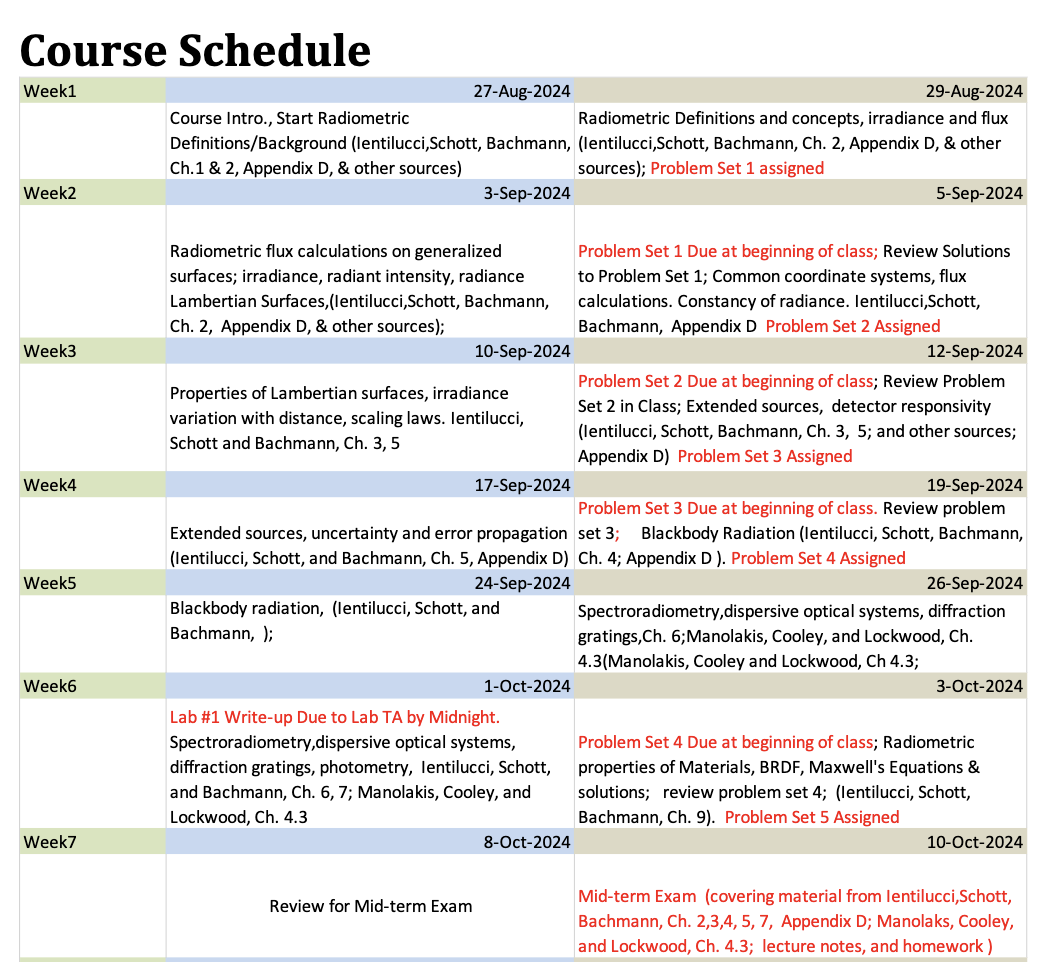
\includegraphics[scale=.95]{Radiometry/Week1/Notes/Syllabus.png}
%\caption{Course Syllabus: He goes through this pretty thoroughly, except that %we did not get to Week 6. The exam is on 2,3,4,5, and 6.}
%\label{fig:Snowman3}
%\end{figure}


\section{Equations}



%\subsection{The Grating Equation}
%Sometimes the given information is in number of grooves or lines per milimeter: lpm 
%$d_{mm} = \frac{1}{lpm}$
%\begin{equation}
%    \Gamma_{Tot}=d(sin \theta_{i} + sin \theta_{r}) = \frac{l}{N}(sin \theta_{i} + sin \theta_{r}) = m \lambda
%\end{equation}
%Where m =0,1,2,3,...

\section{HANA Tree and Marsh Study}
\clearpage
More pictures are available and in the repository of this LaTeX file. 
\begin{figure}[h!]
\centering
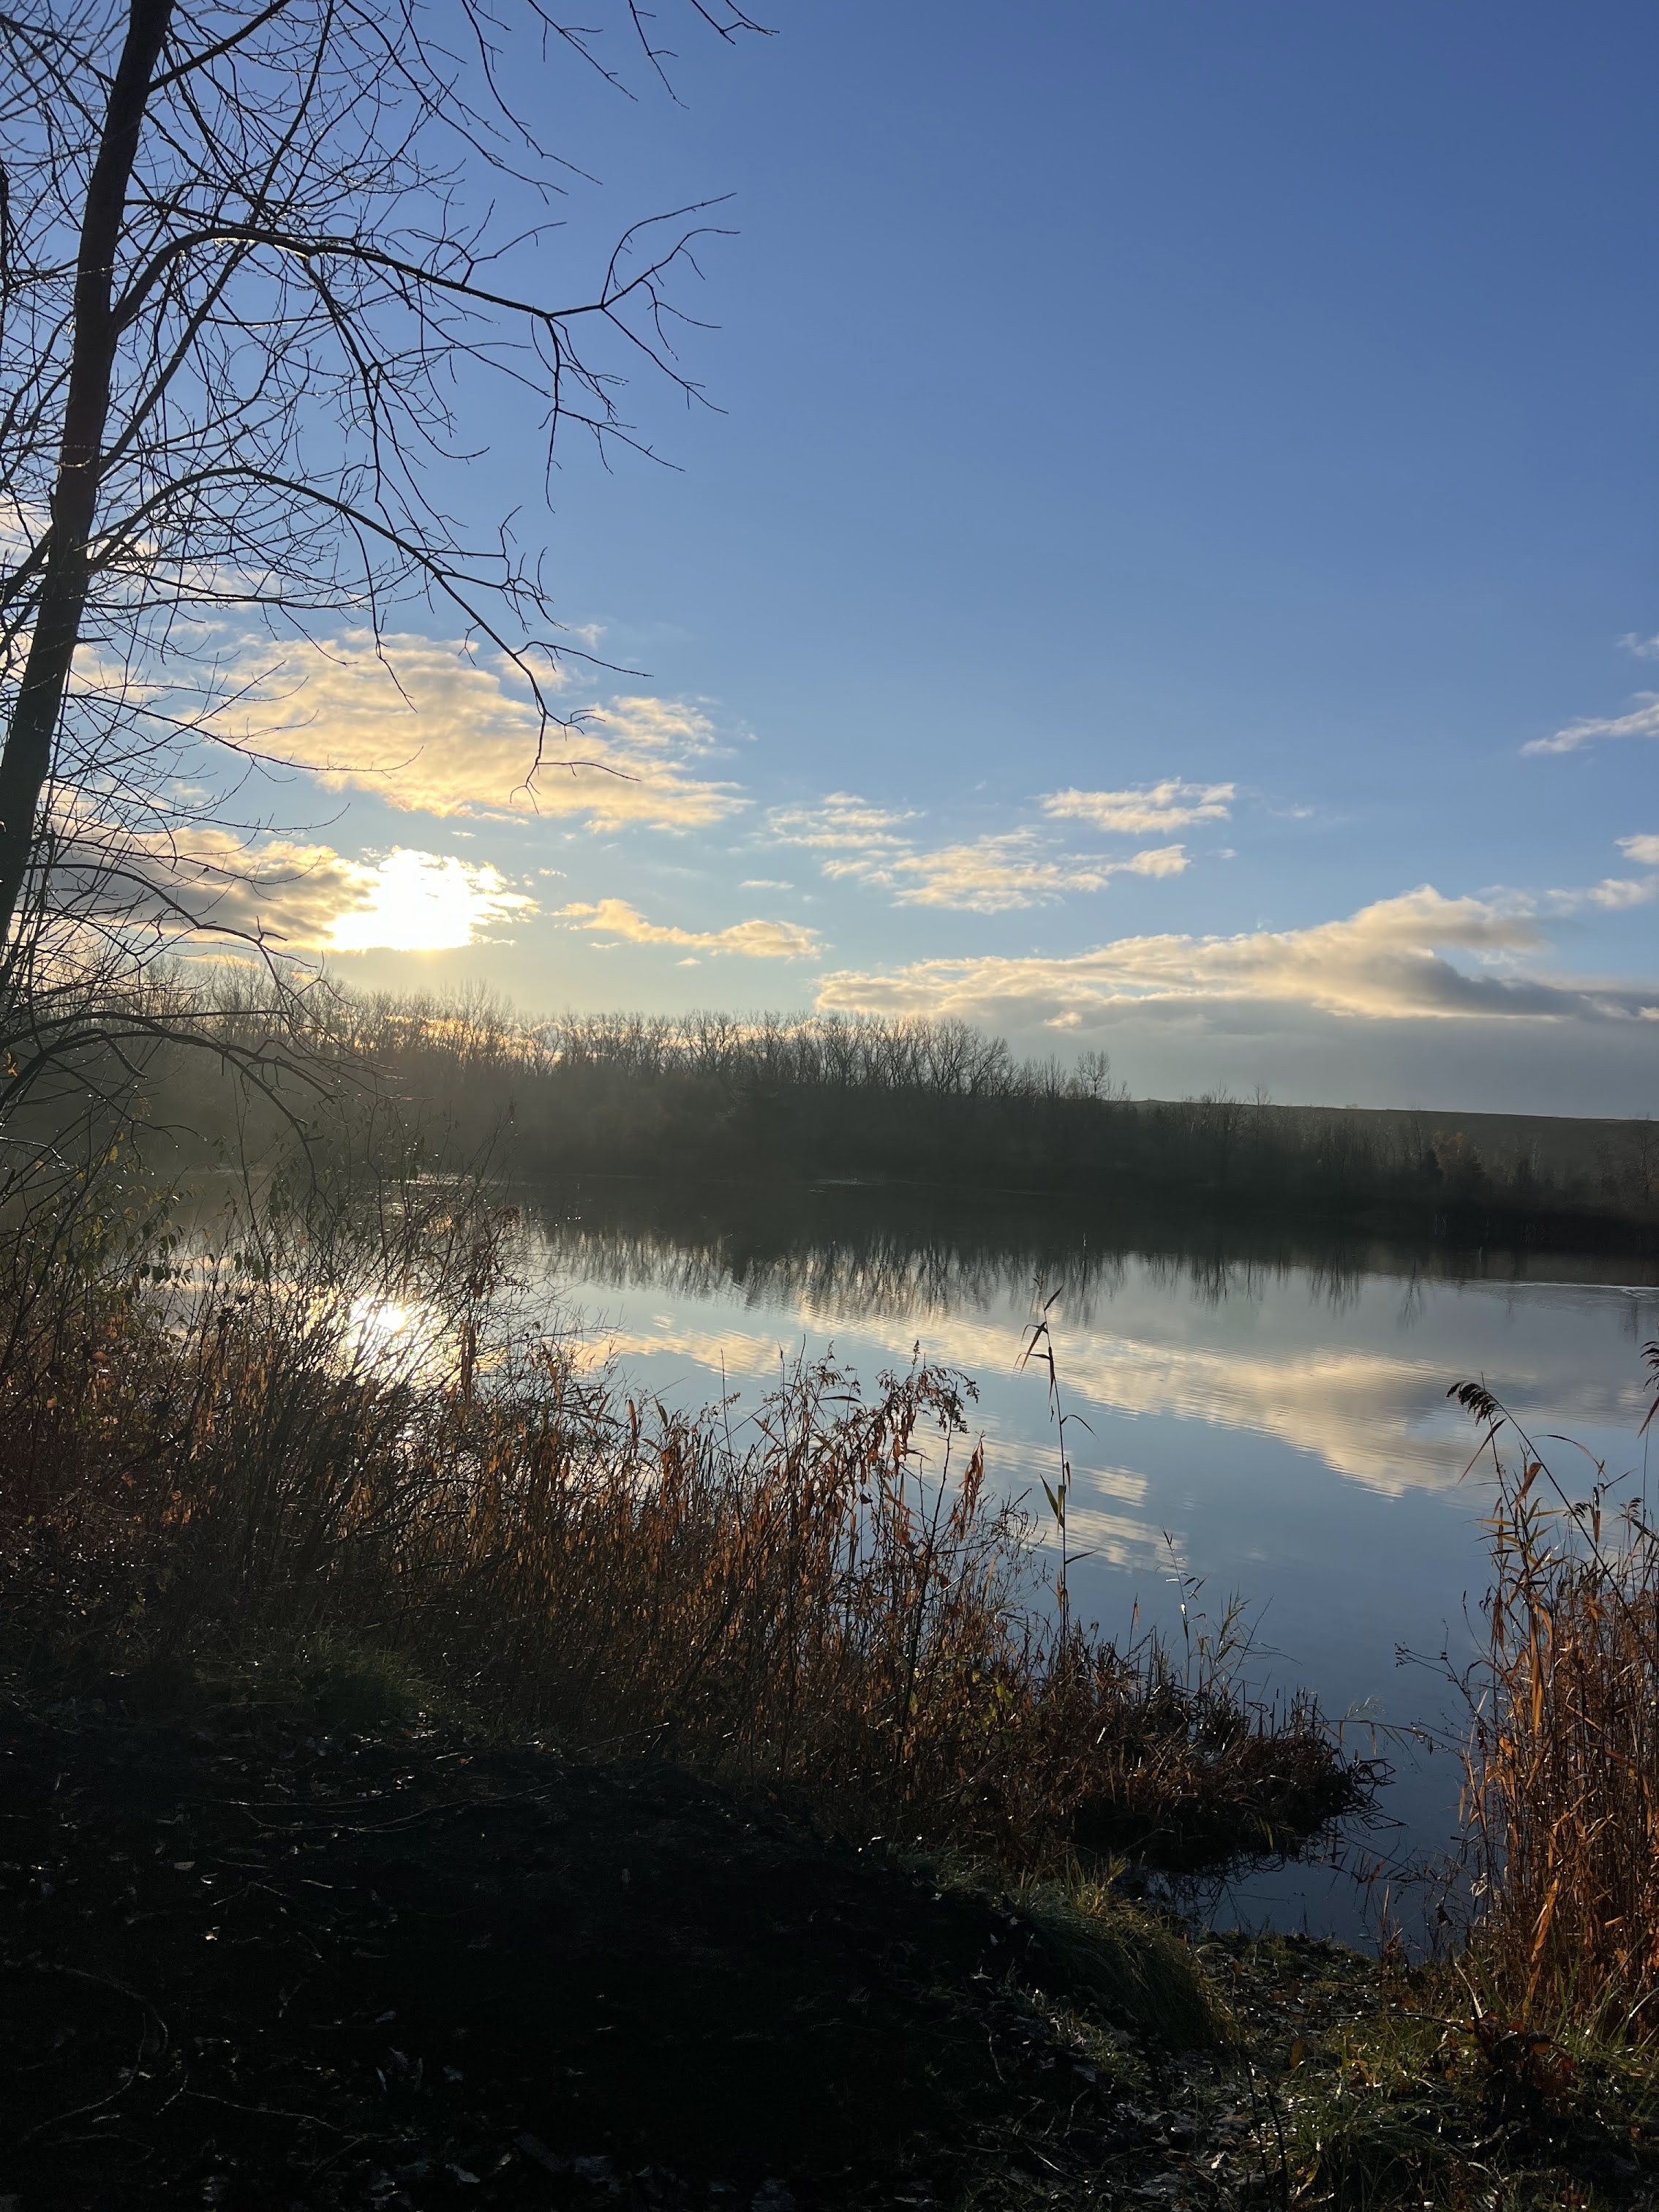
\includegraphics[scale=.1]{Research/HANA/NOV2024/IMG_9791.JPG}
\caption{HANA Tree Study}
\label{fig:HANA}
\end{figure}



\begin{figure}[h!]
\centering
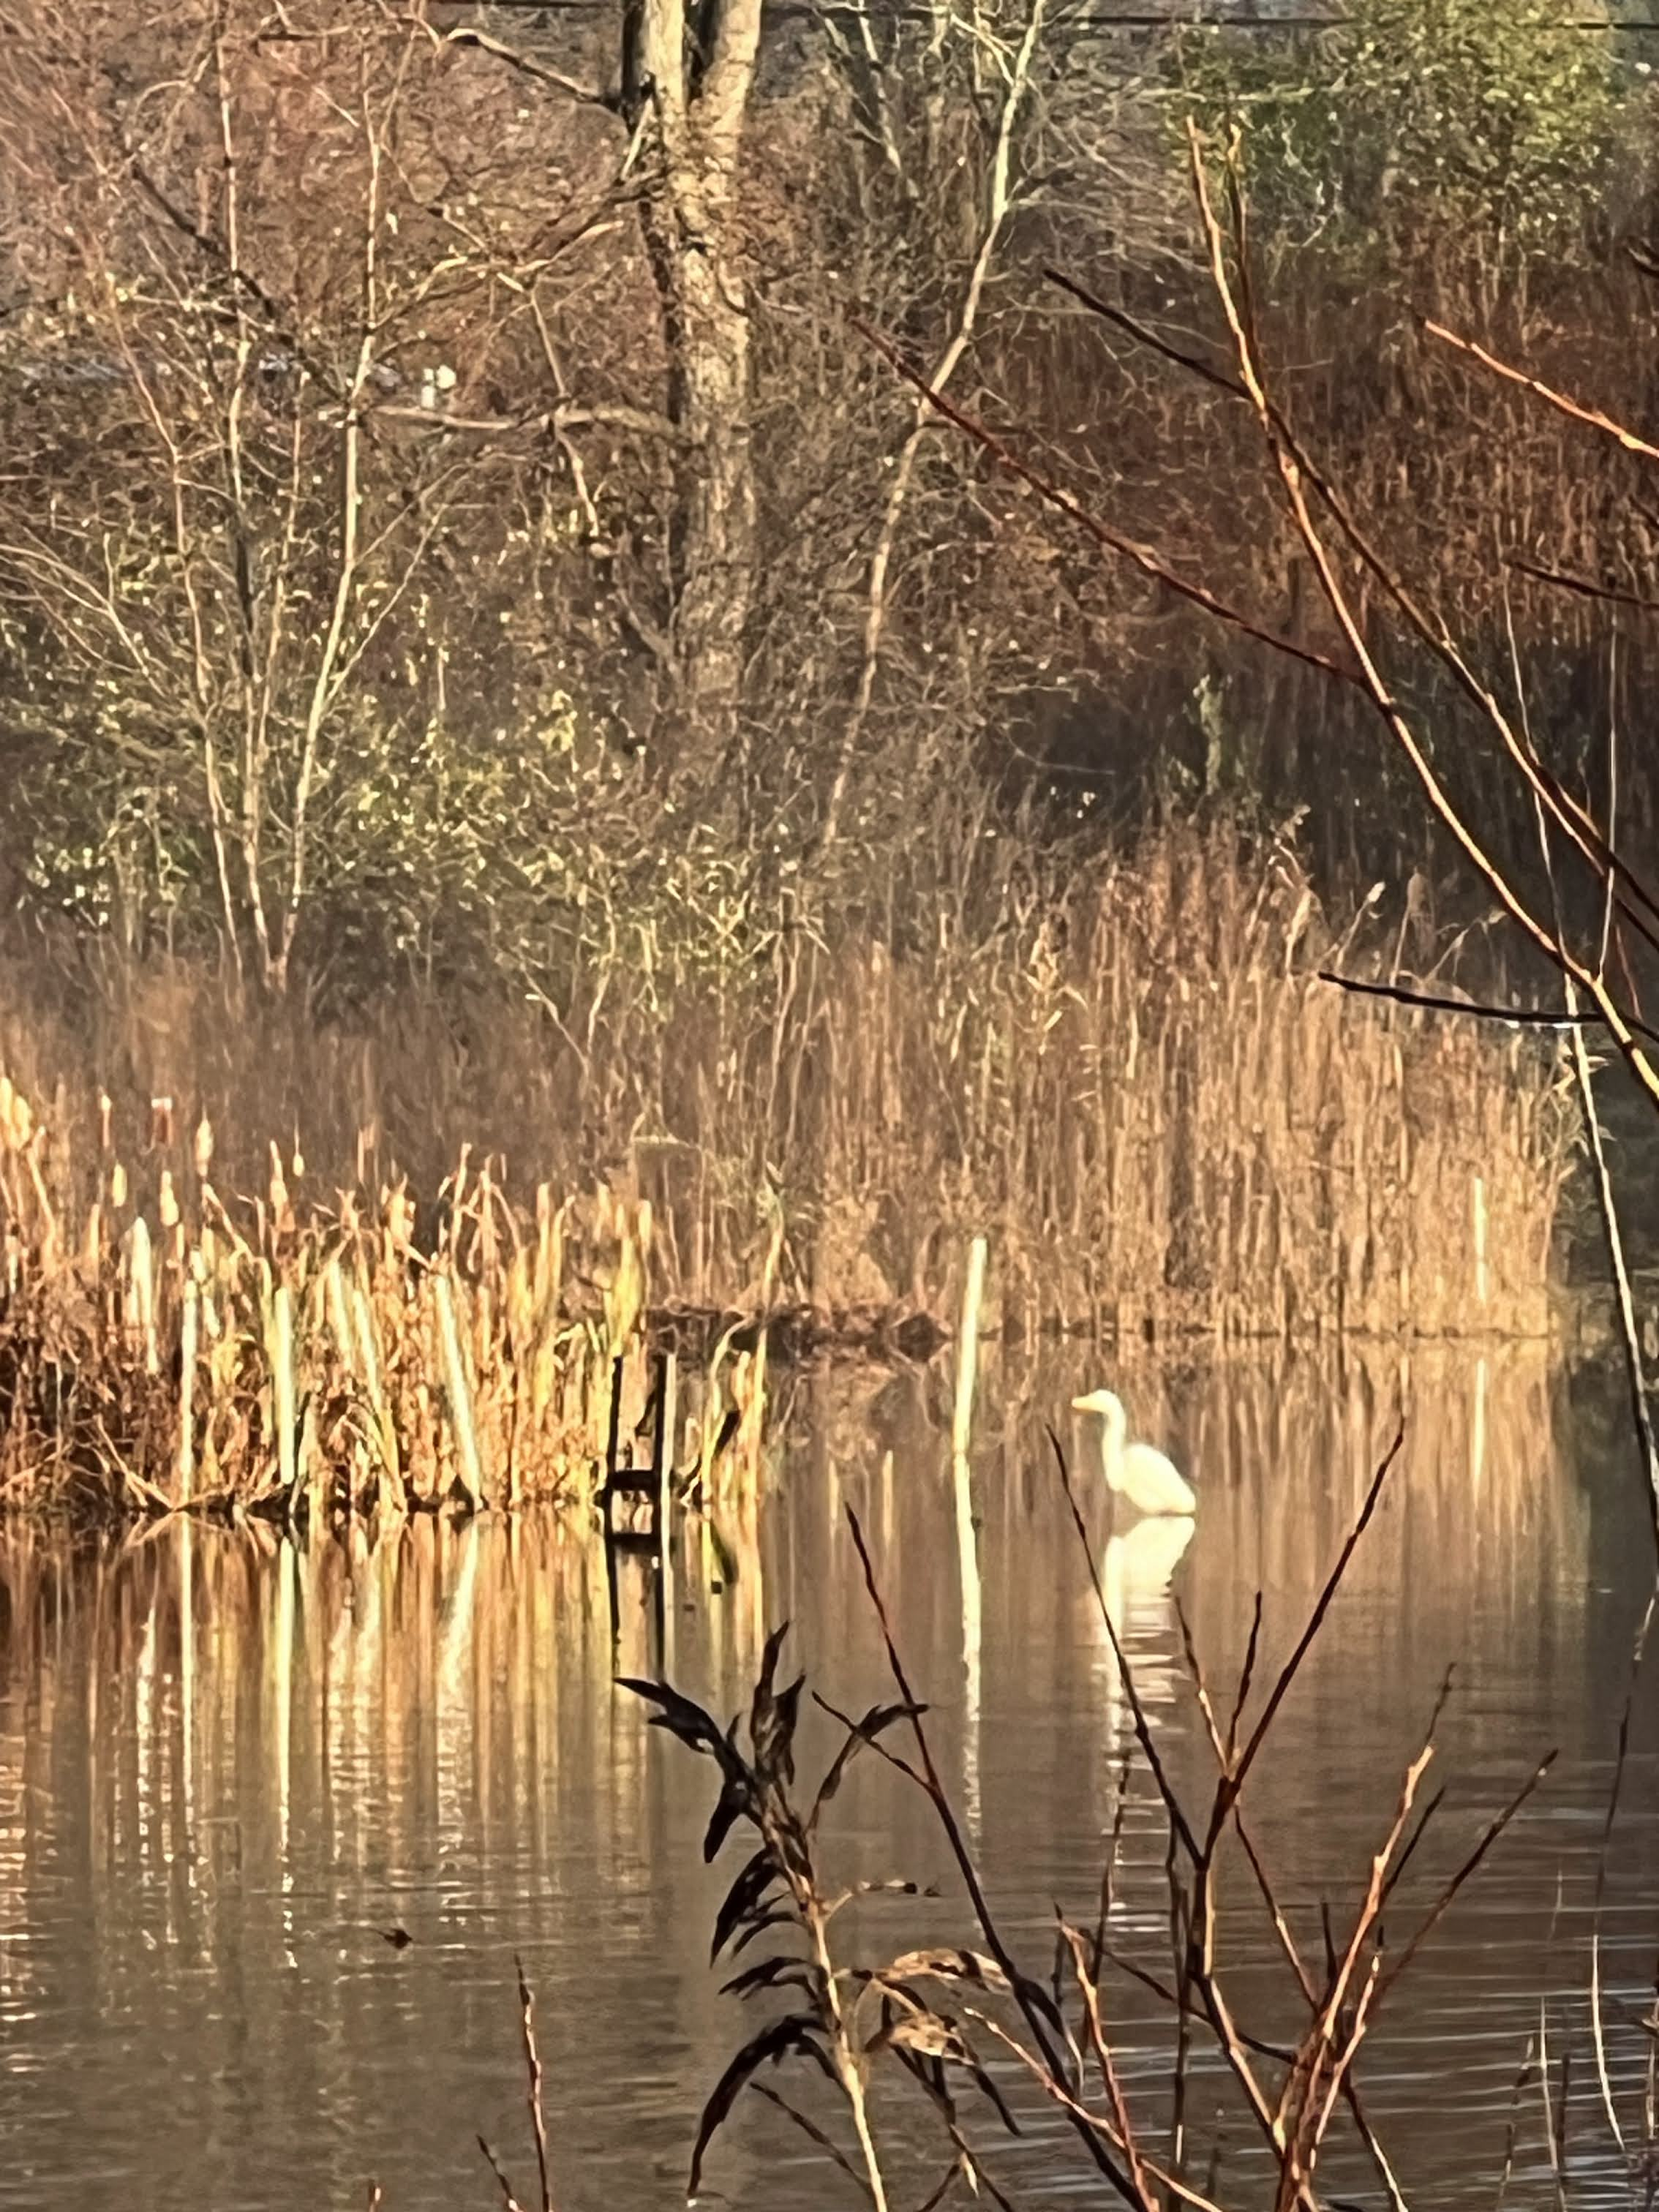
\includegraphics[scale=.1]{Research/HANA/NOV2024/IMG_9800.JPG}
\caption{HANA Tree Study}
\label{fig:HANA}
\end{figure}

\begin{figure}[h!]
\centering
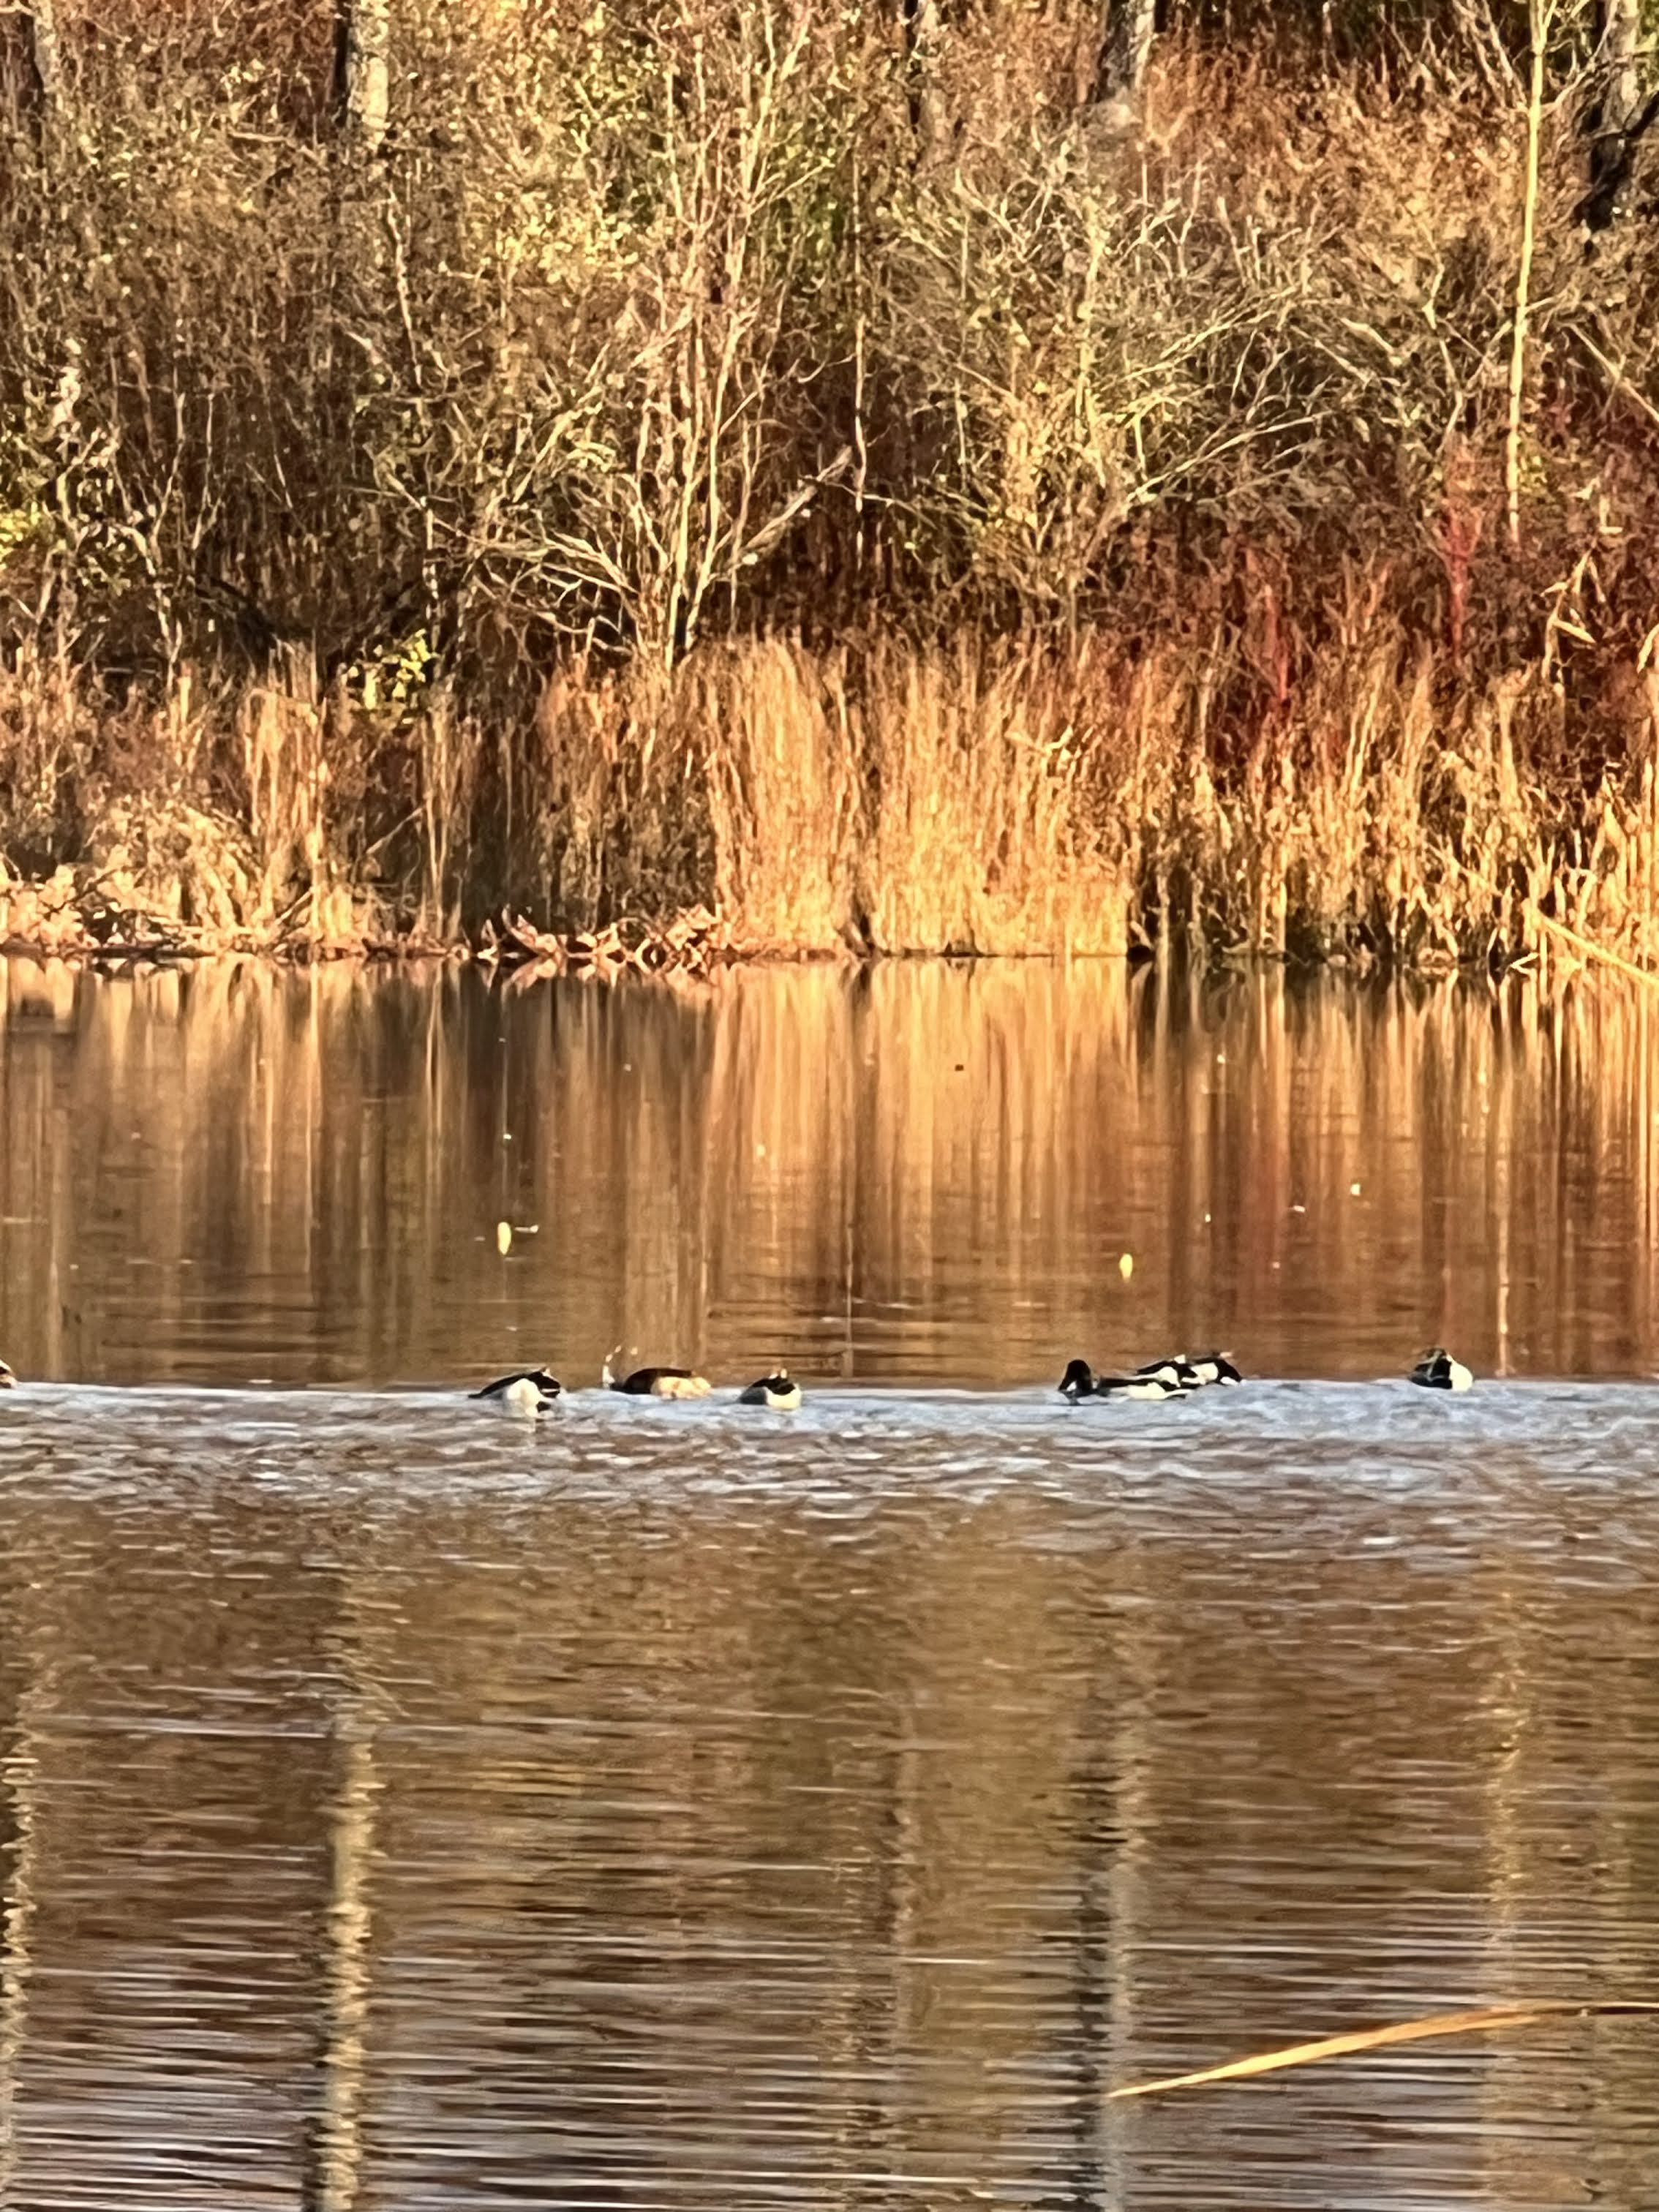
\includegraphics[scale=.1]{Research/HANA/NOV2024/IMG_9811.JPG}
\caption{HANA Tree Study}
\label{fig:HANA}
\end{figure}

\begin{figure}[h!]
\centering
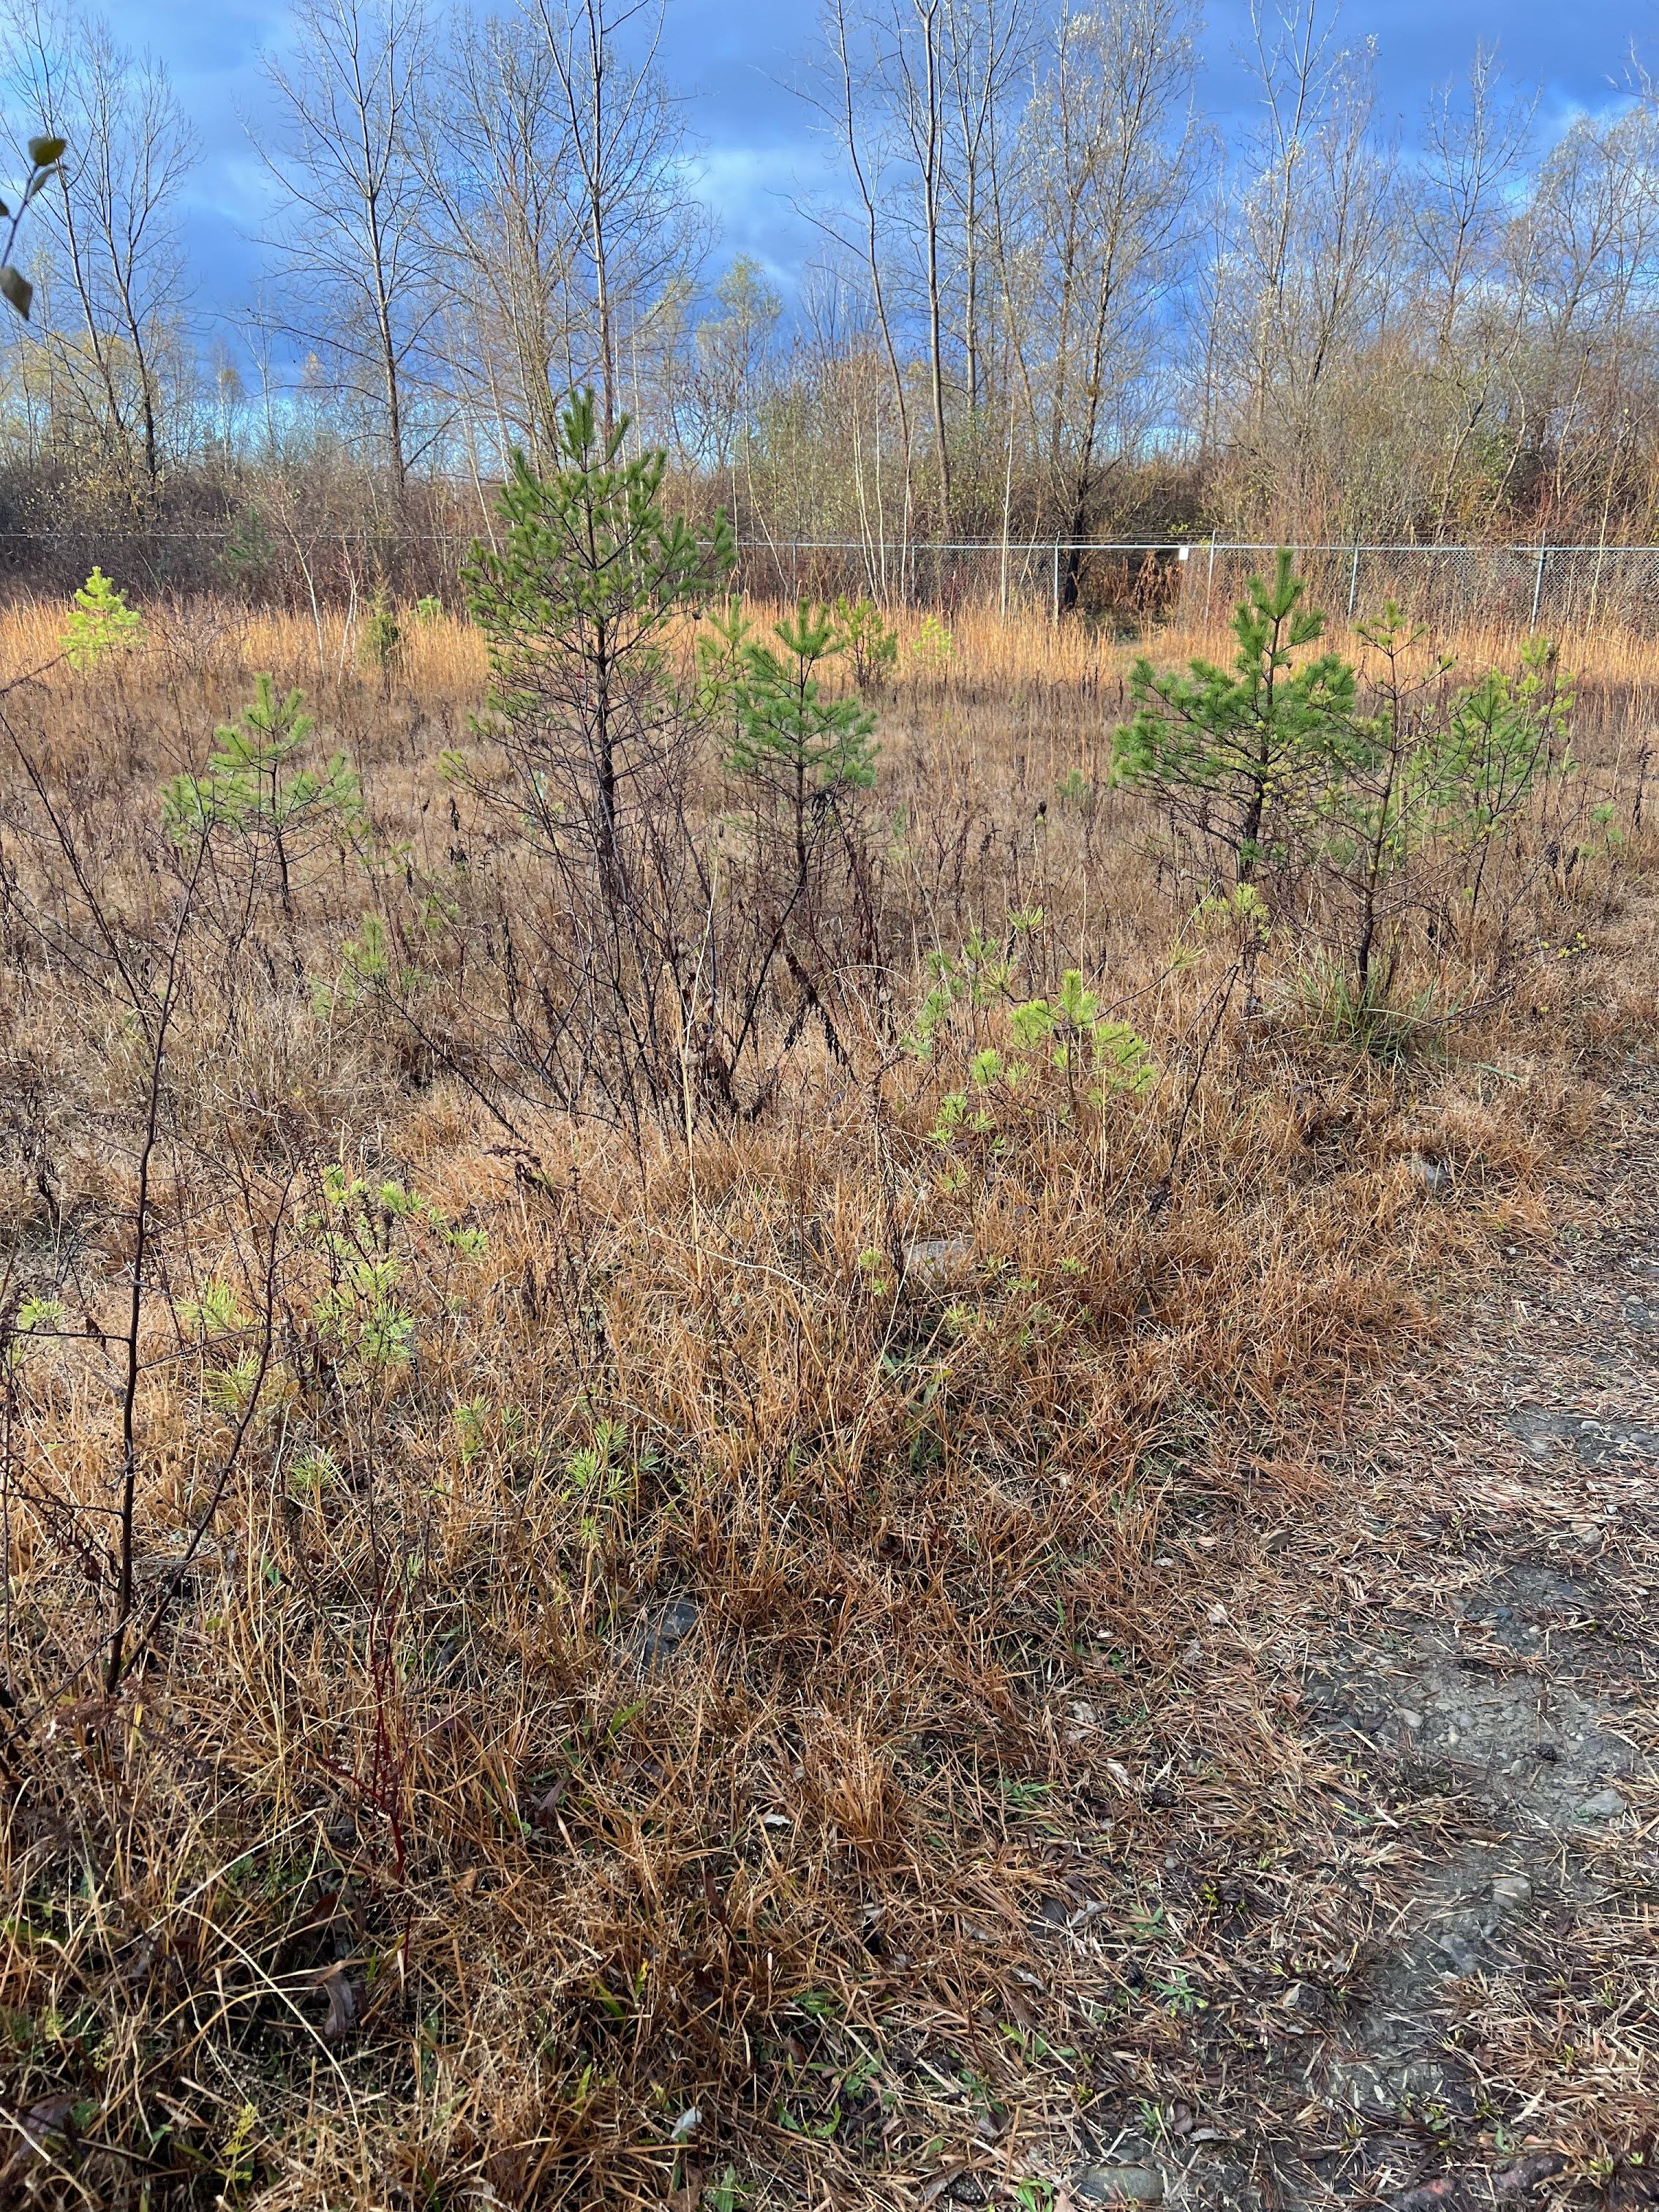
\includegraphics[scale=.1]{Research/HANA/NOV2024/IMG_9820.JPG}
\caption{HANA Tree Study}
\label{fig:HANA}
\end{figure}

\begin{figure}[h!]
\centering
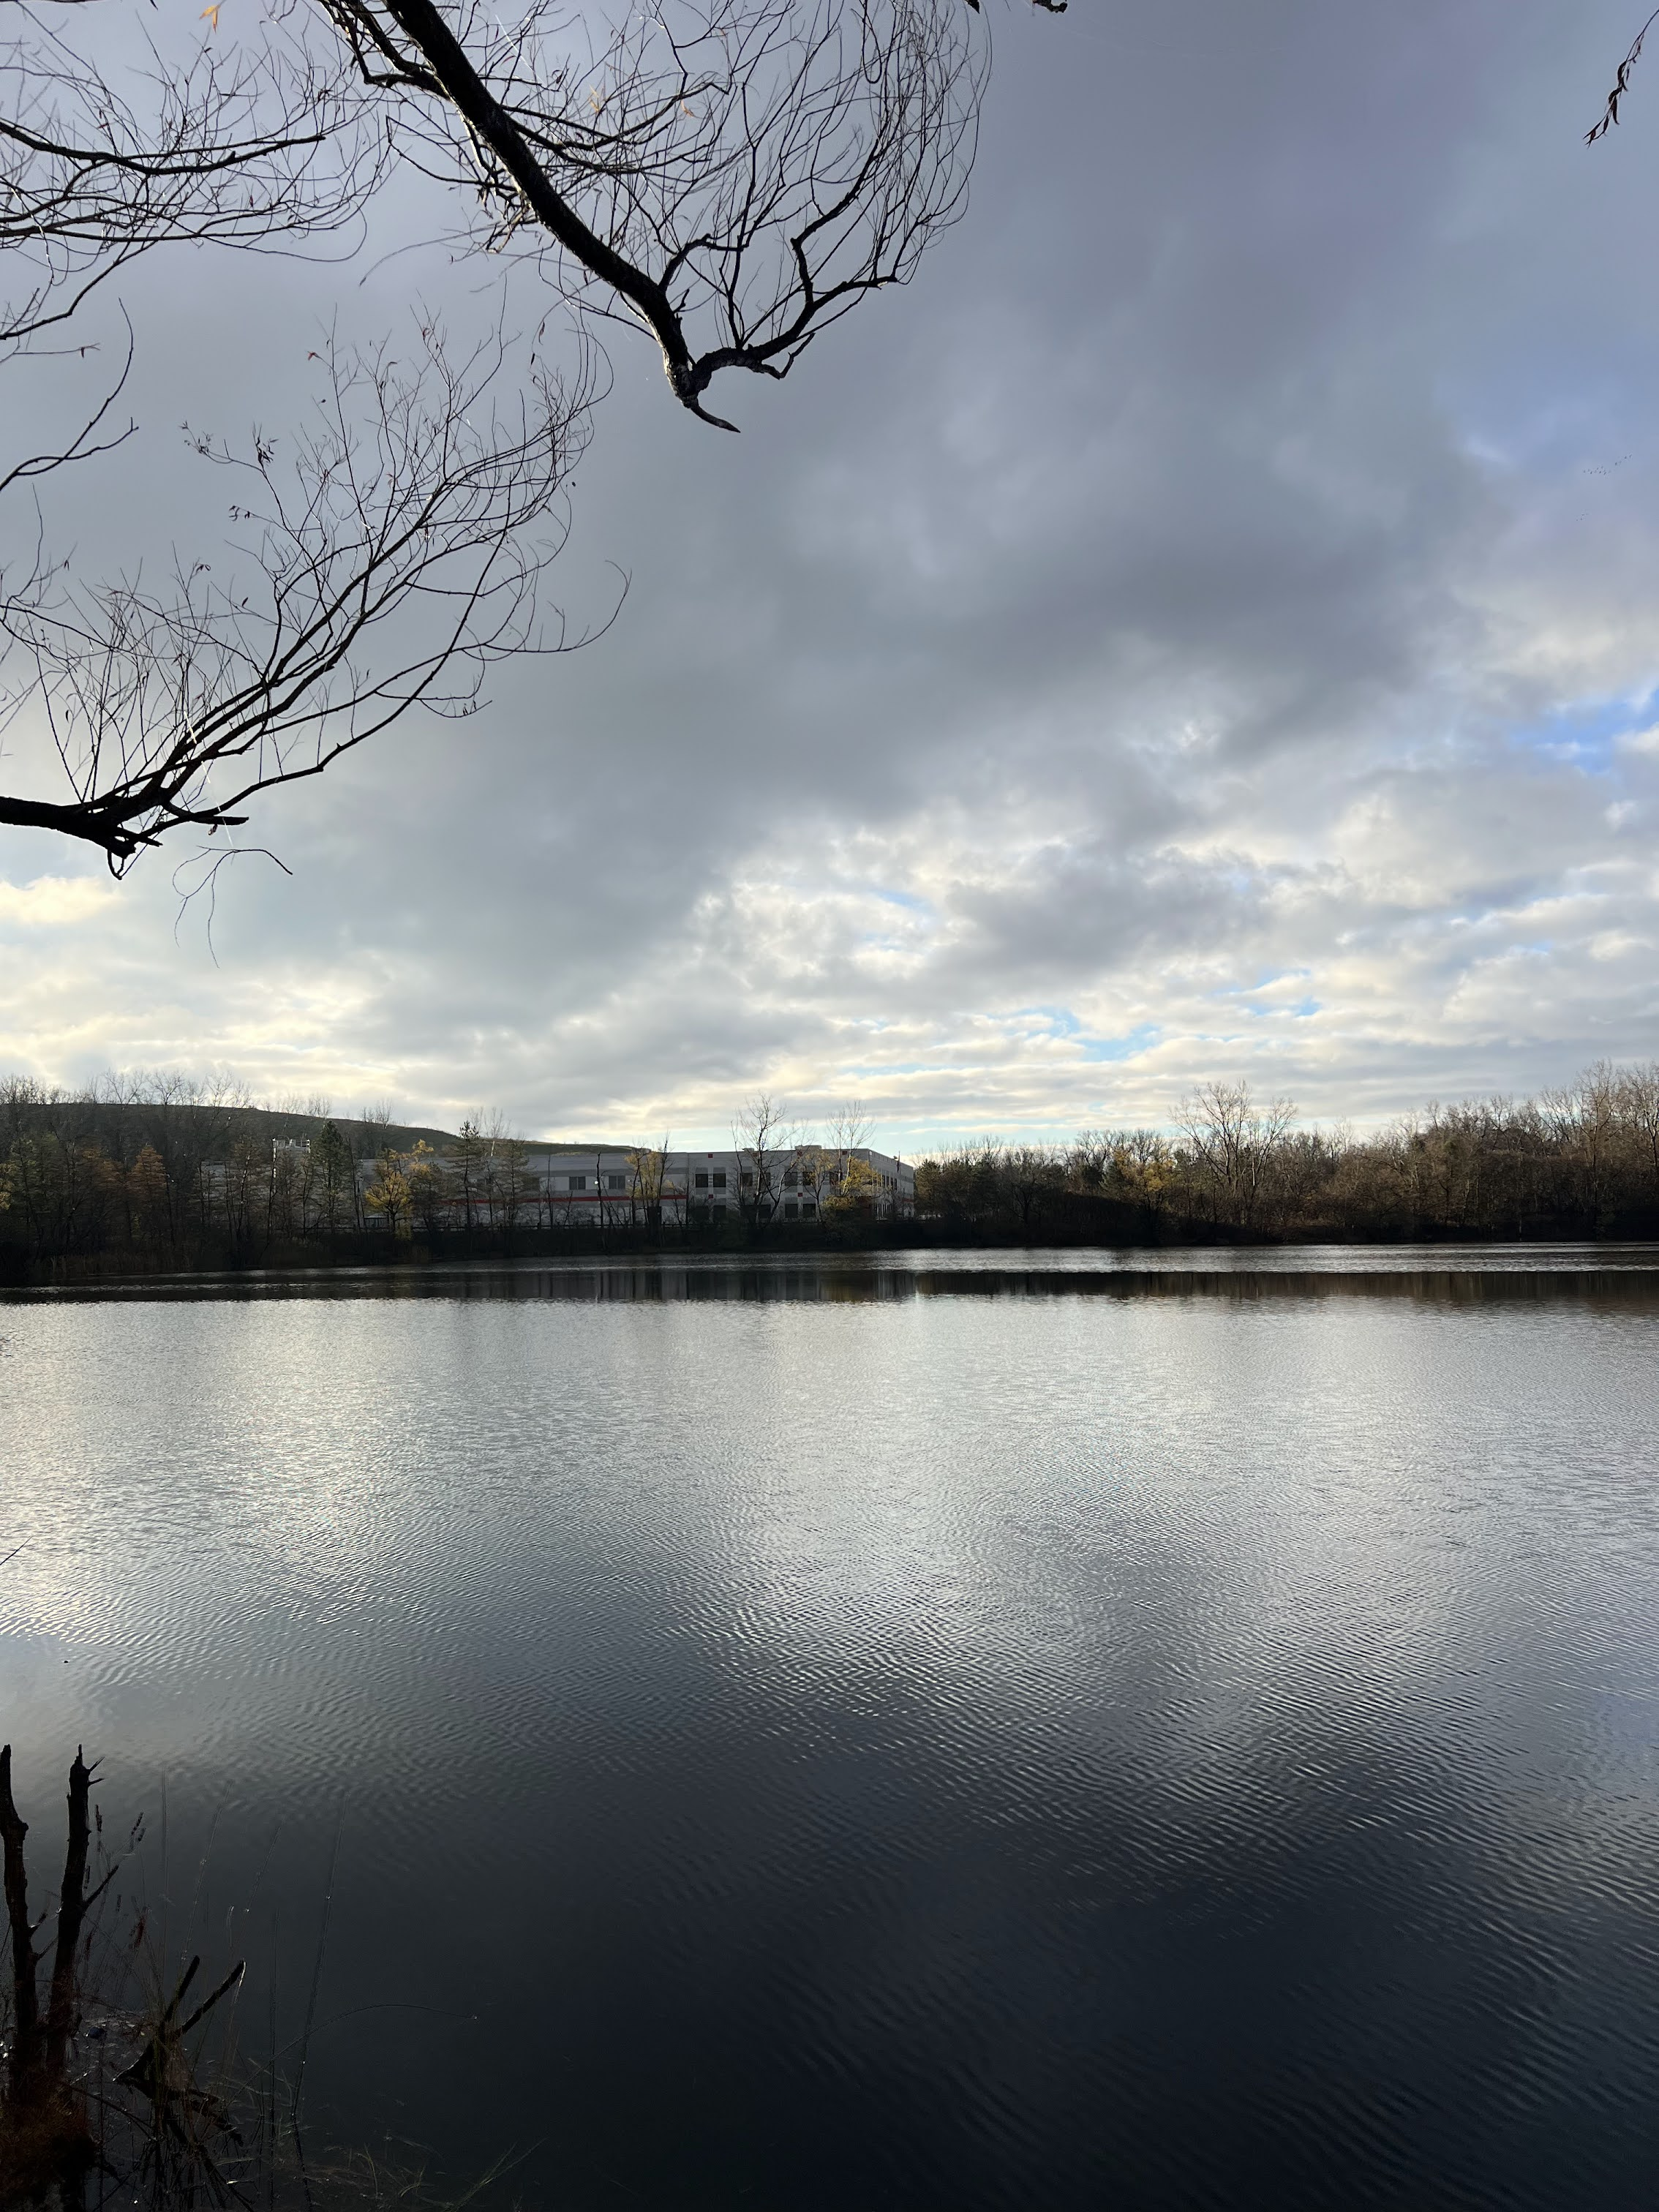
\includegraphics[scale=.1]{Research/HANA/NOV2024/IMG_9830.JPG}
\caption{HANA Tree Study}
\label{fig:HANA}
\end{figure}

\begin{figure}[h!]
\centering
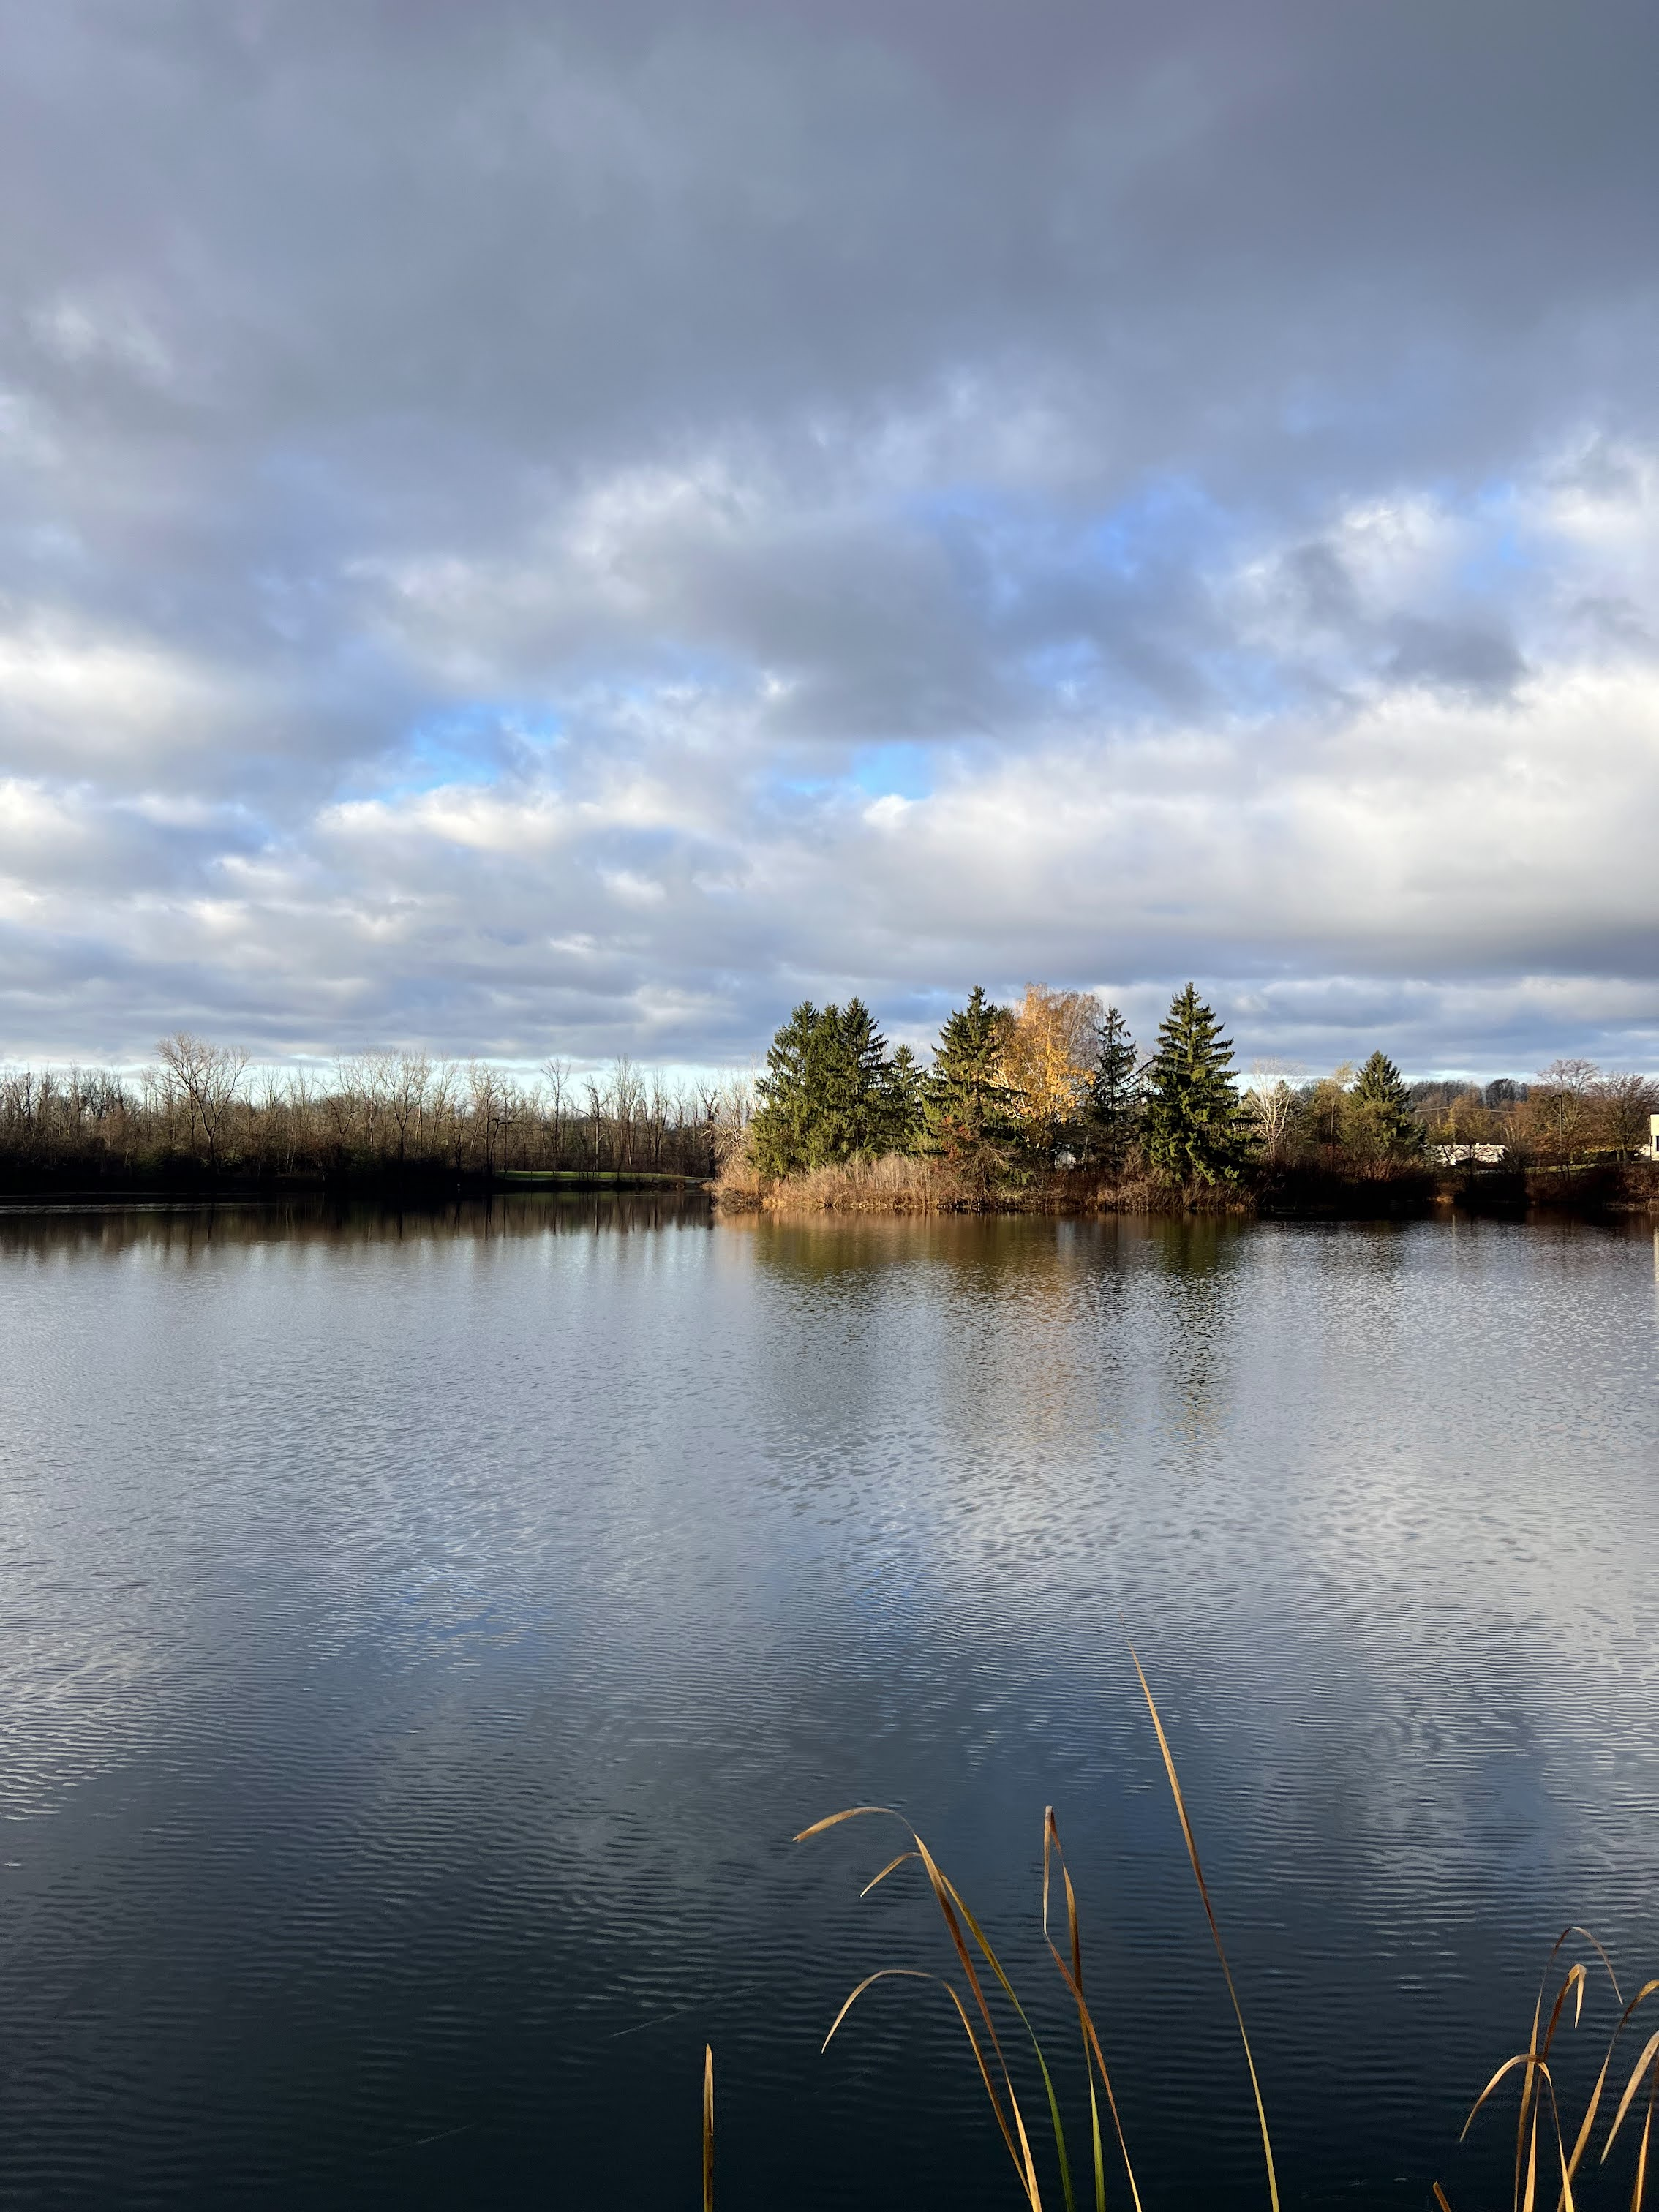
\includegraphics[scale=.1]{Research/HANA/NOV2024/IMG_9834.JPG}
\caption{HANA Tree Study}
\label{fig:HANA}
\end{figure}

\begin{figure}[h!]
\centering
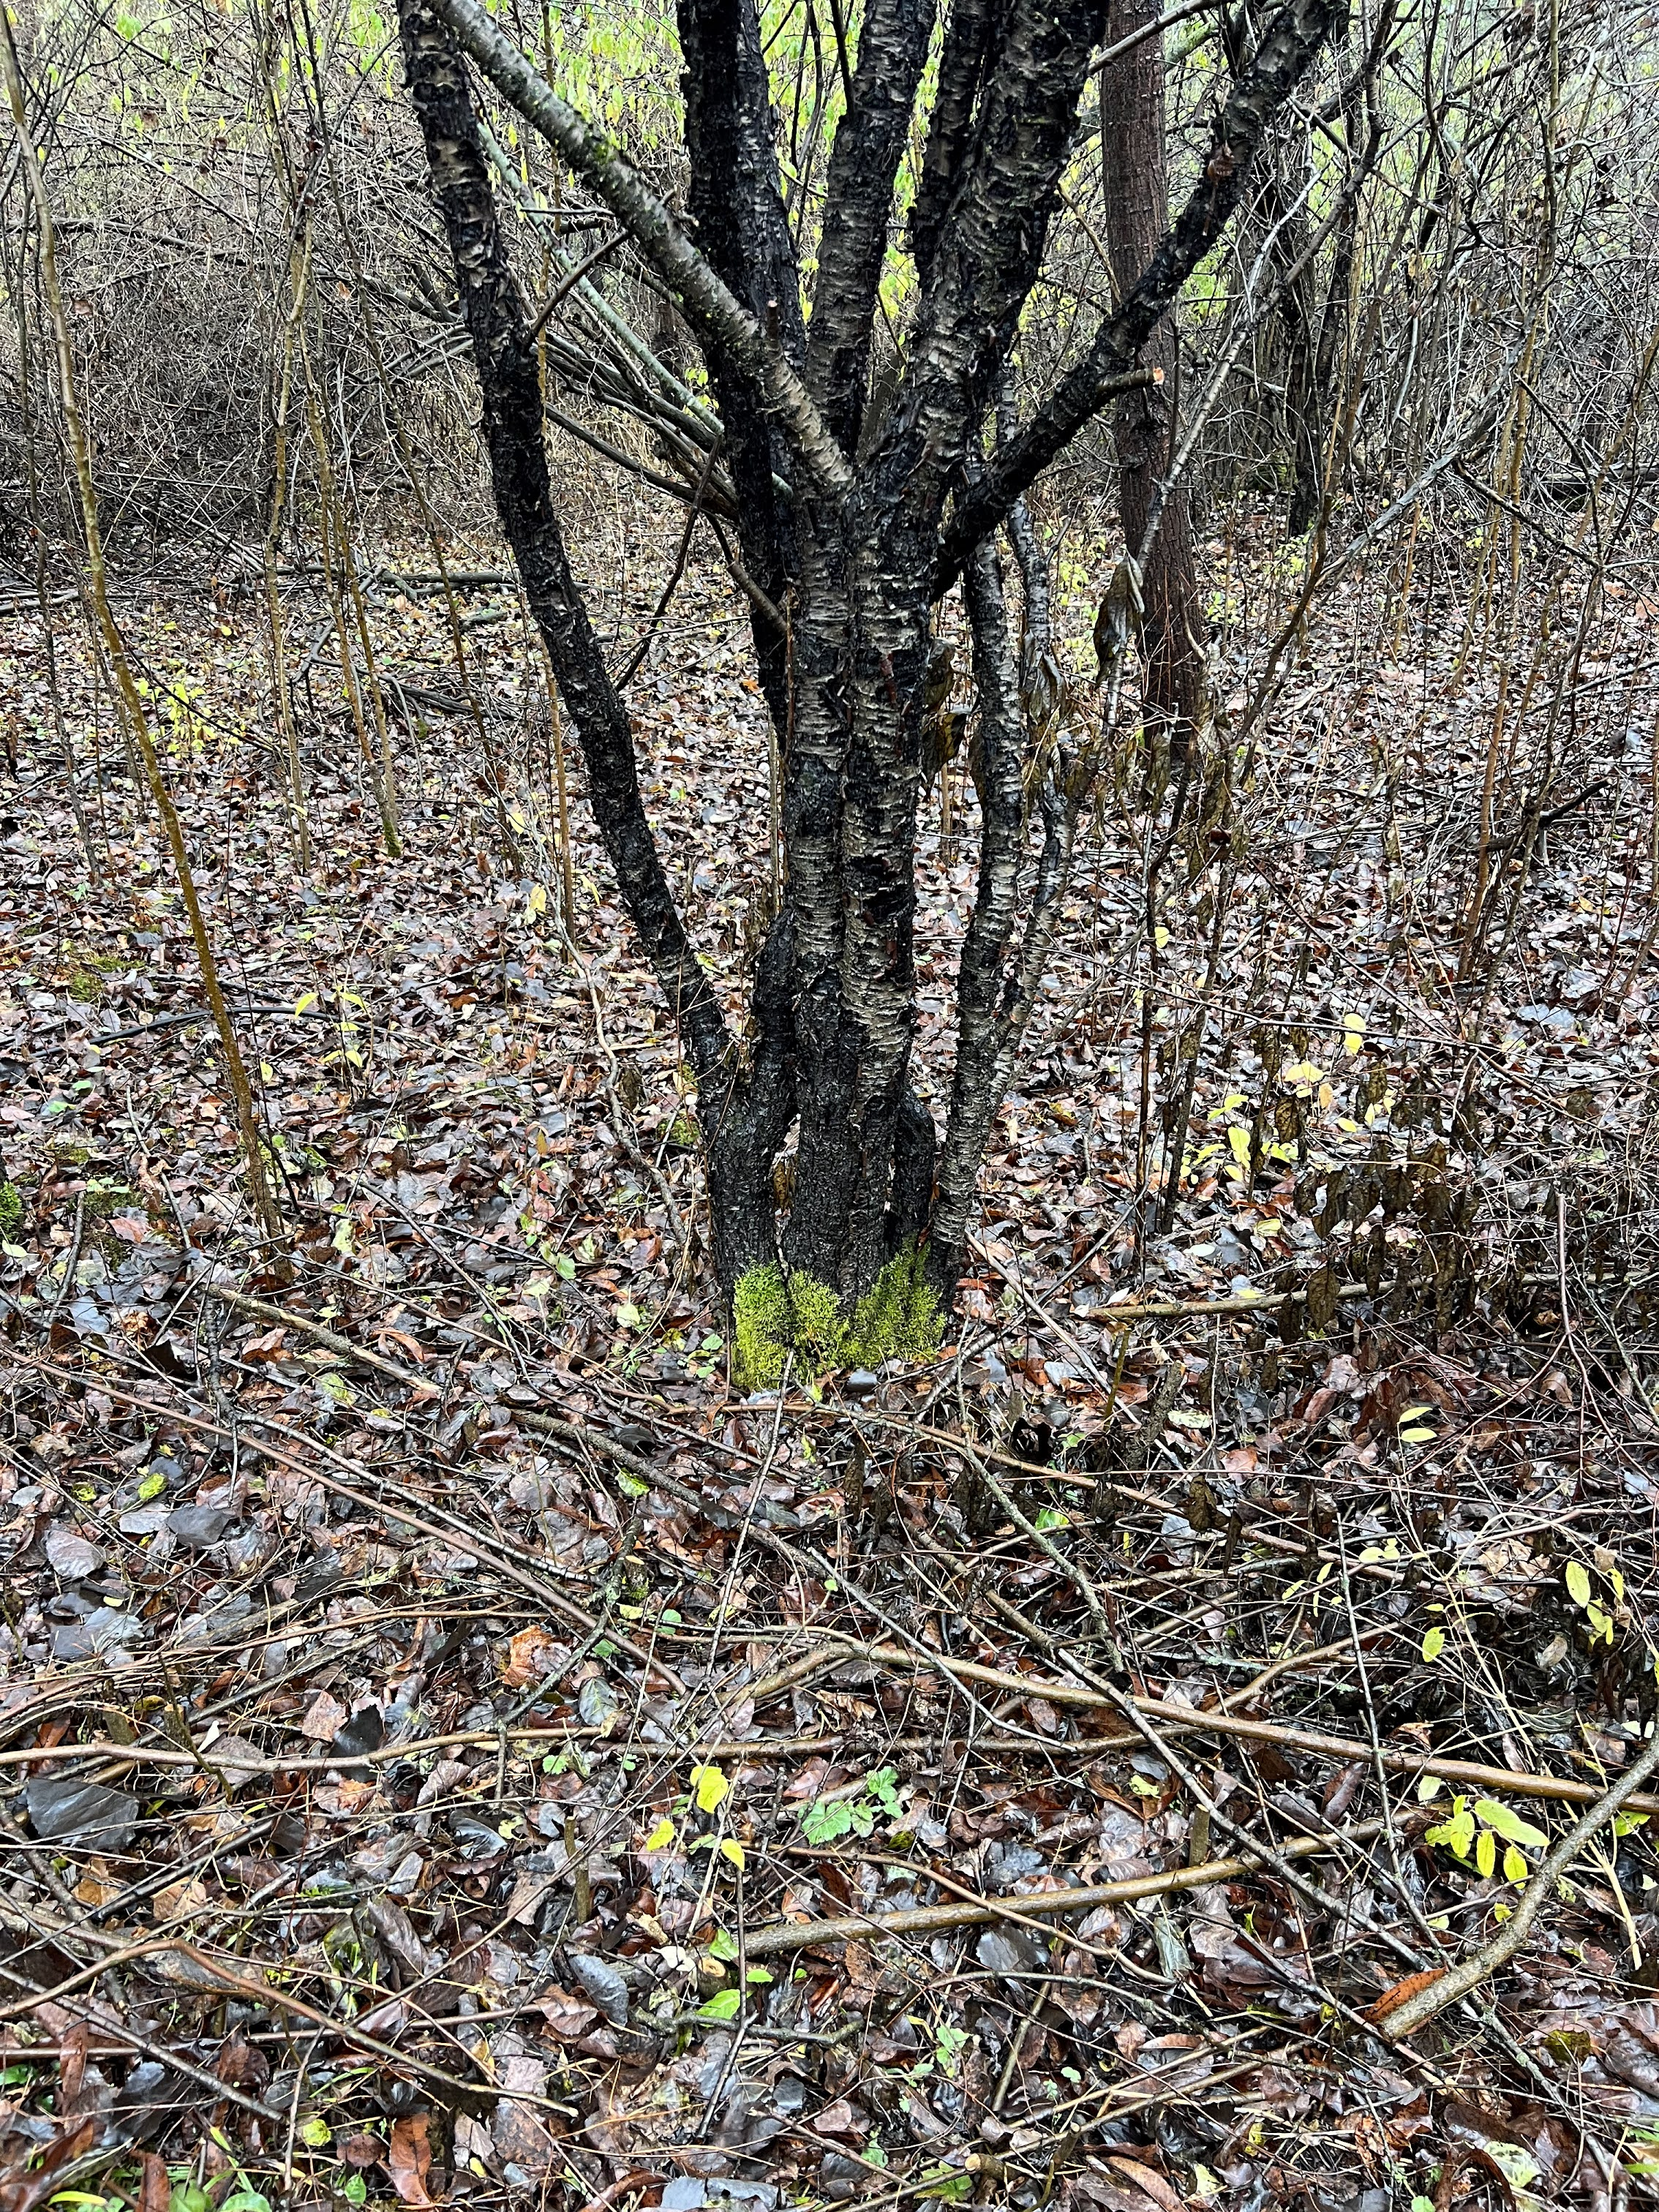
\includegraphics[scale=.1]{Research/HANA/NOV2024/IMG_9845.JPG}
\caption{HANA Tree Study}
\label{fig:HANA}
\end{figure}



\begin{figure}[h!]
\centering
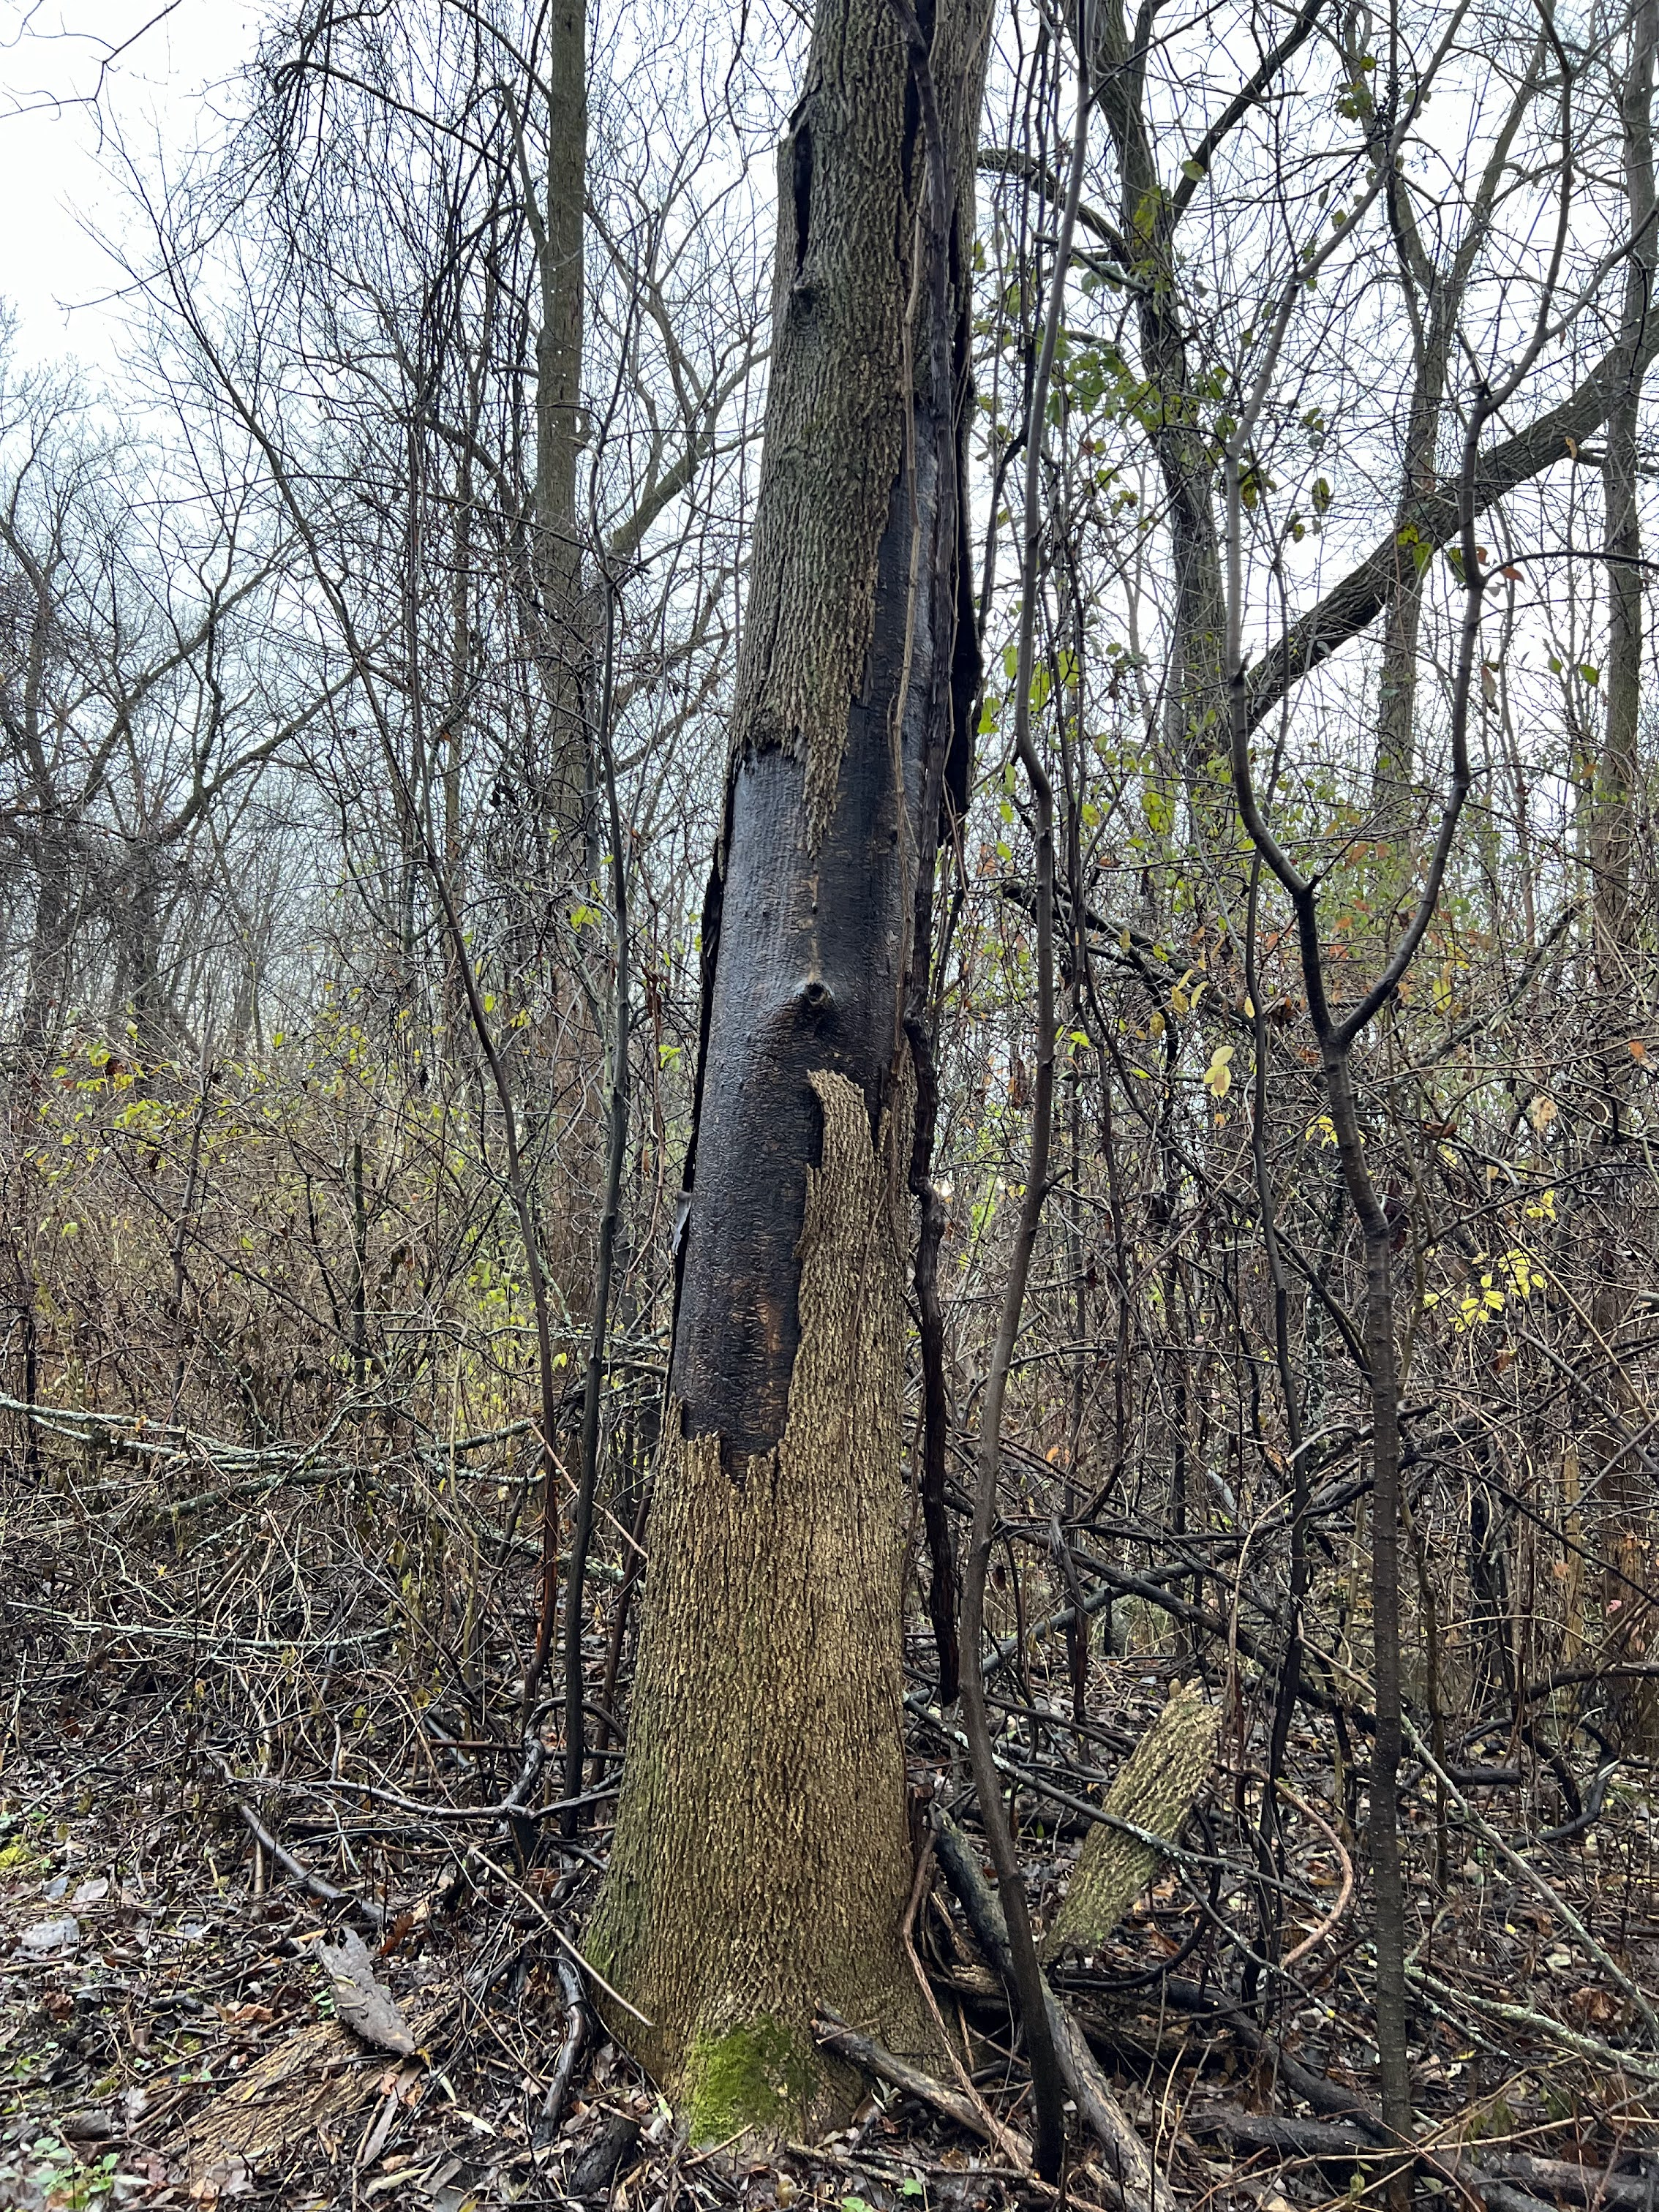
\includegraphics[scale=.1]{Research/HANA/NOV2024/IMG_9848.JPG}
\caption{HANA Tree Study}
\label{fig:HANA}
\end{figure}


\begin{figure}[h!]
\centering
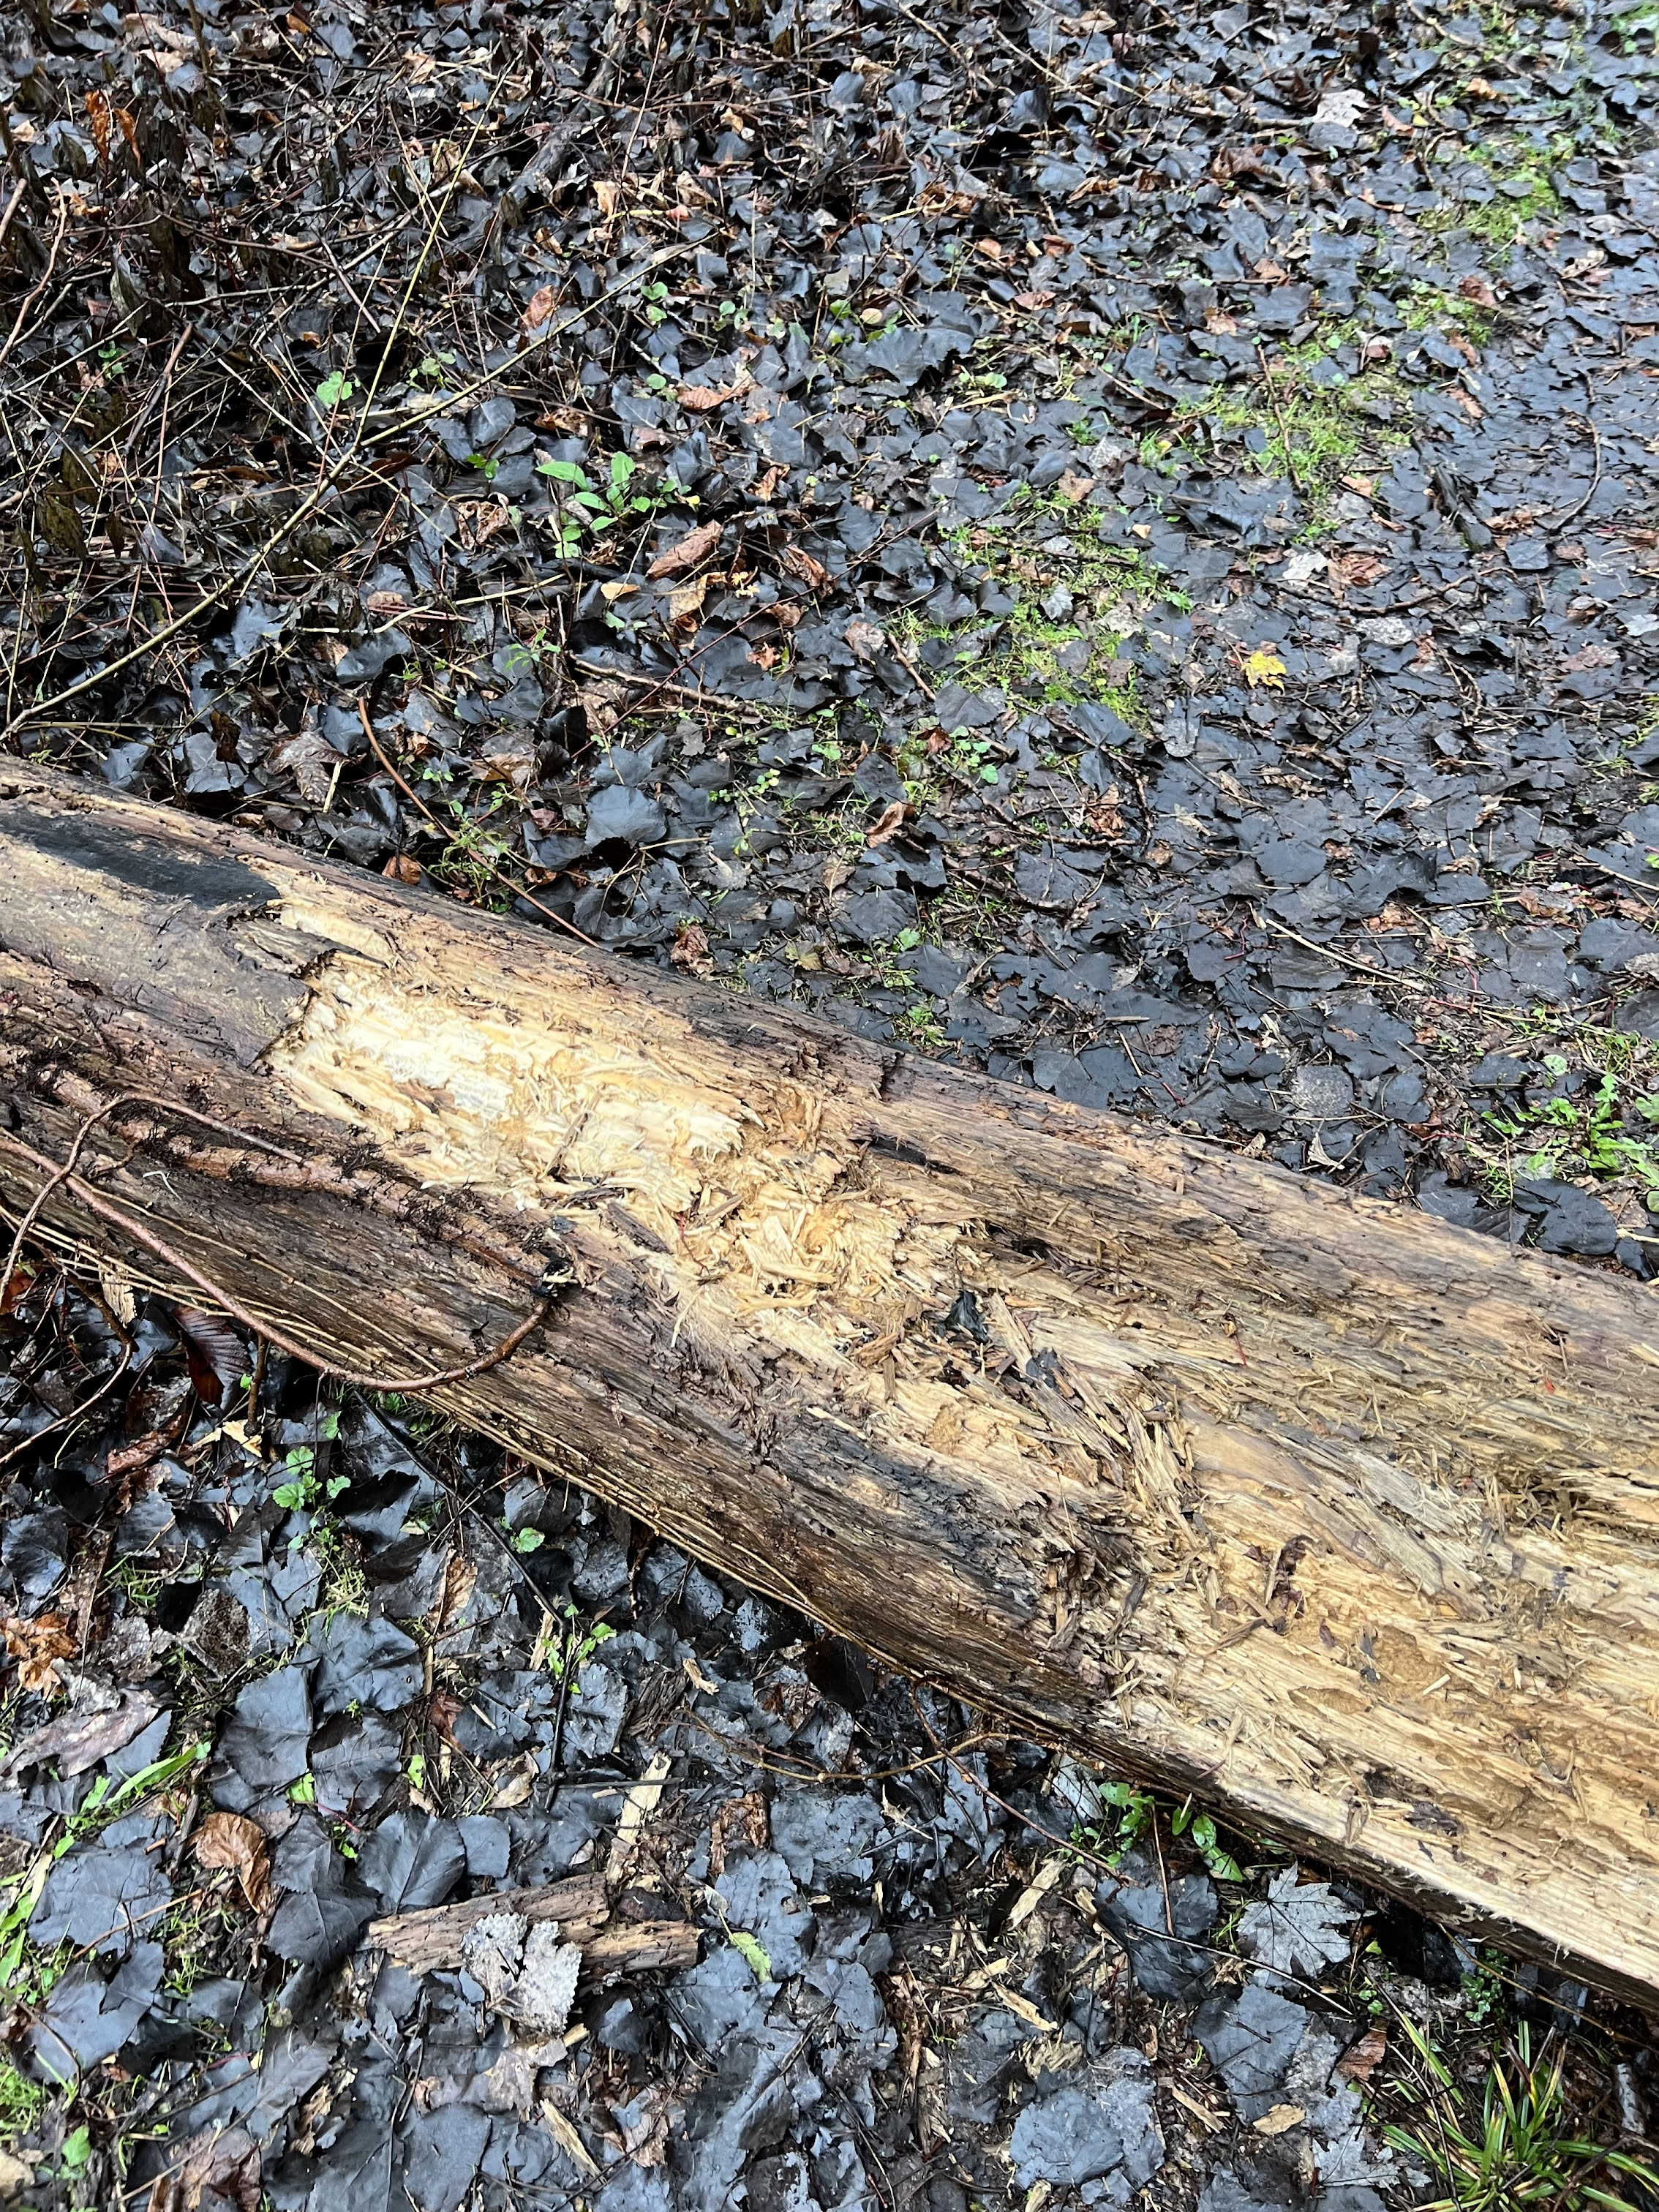
\includegraphics[scale=.1]{Research/HANA/NOV2024/IMG_9852.JPG}
\caption{HANA Tree Study}
\label{fig:HANA}
\end{figure}



\begin{figure}[h!]
\centering
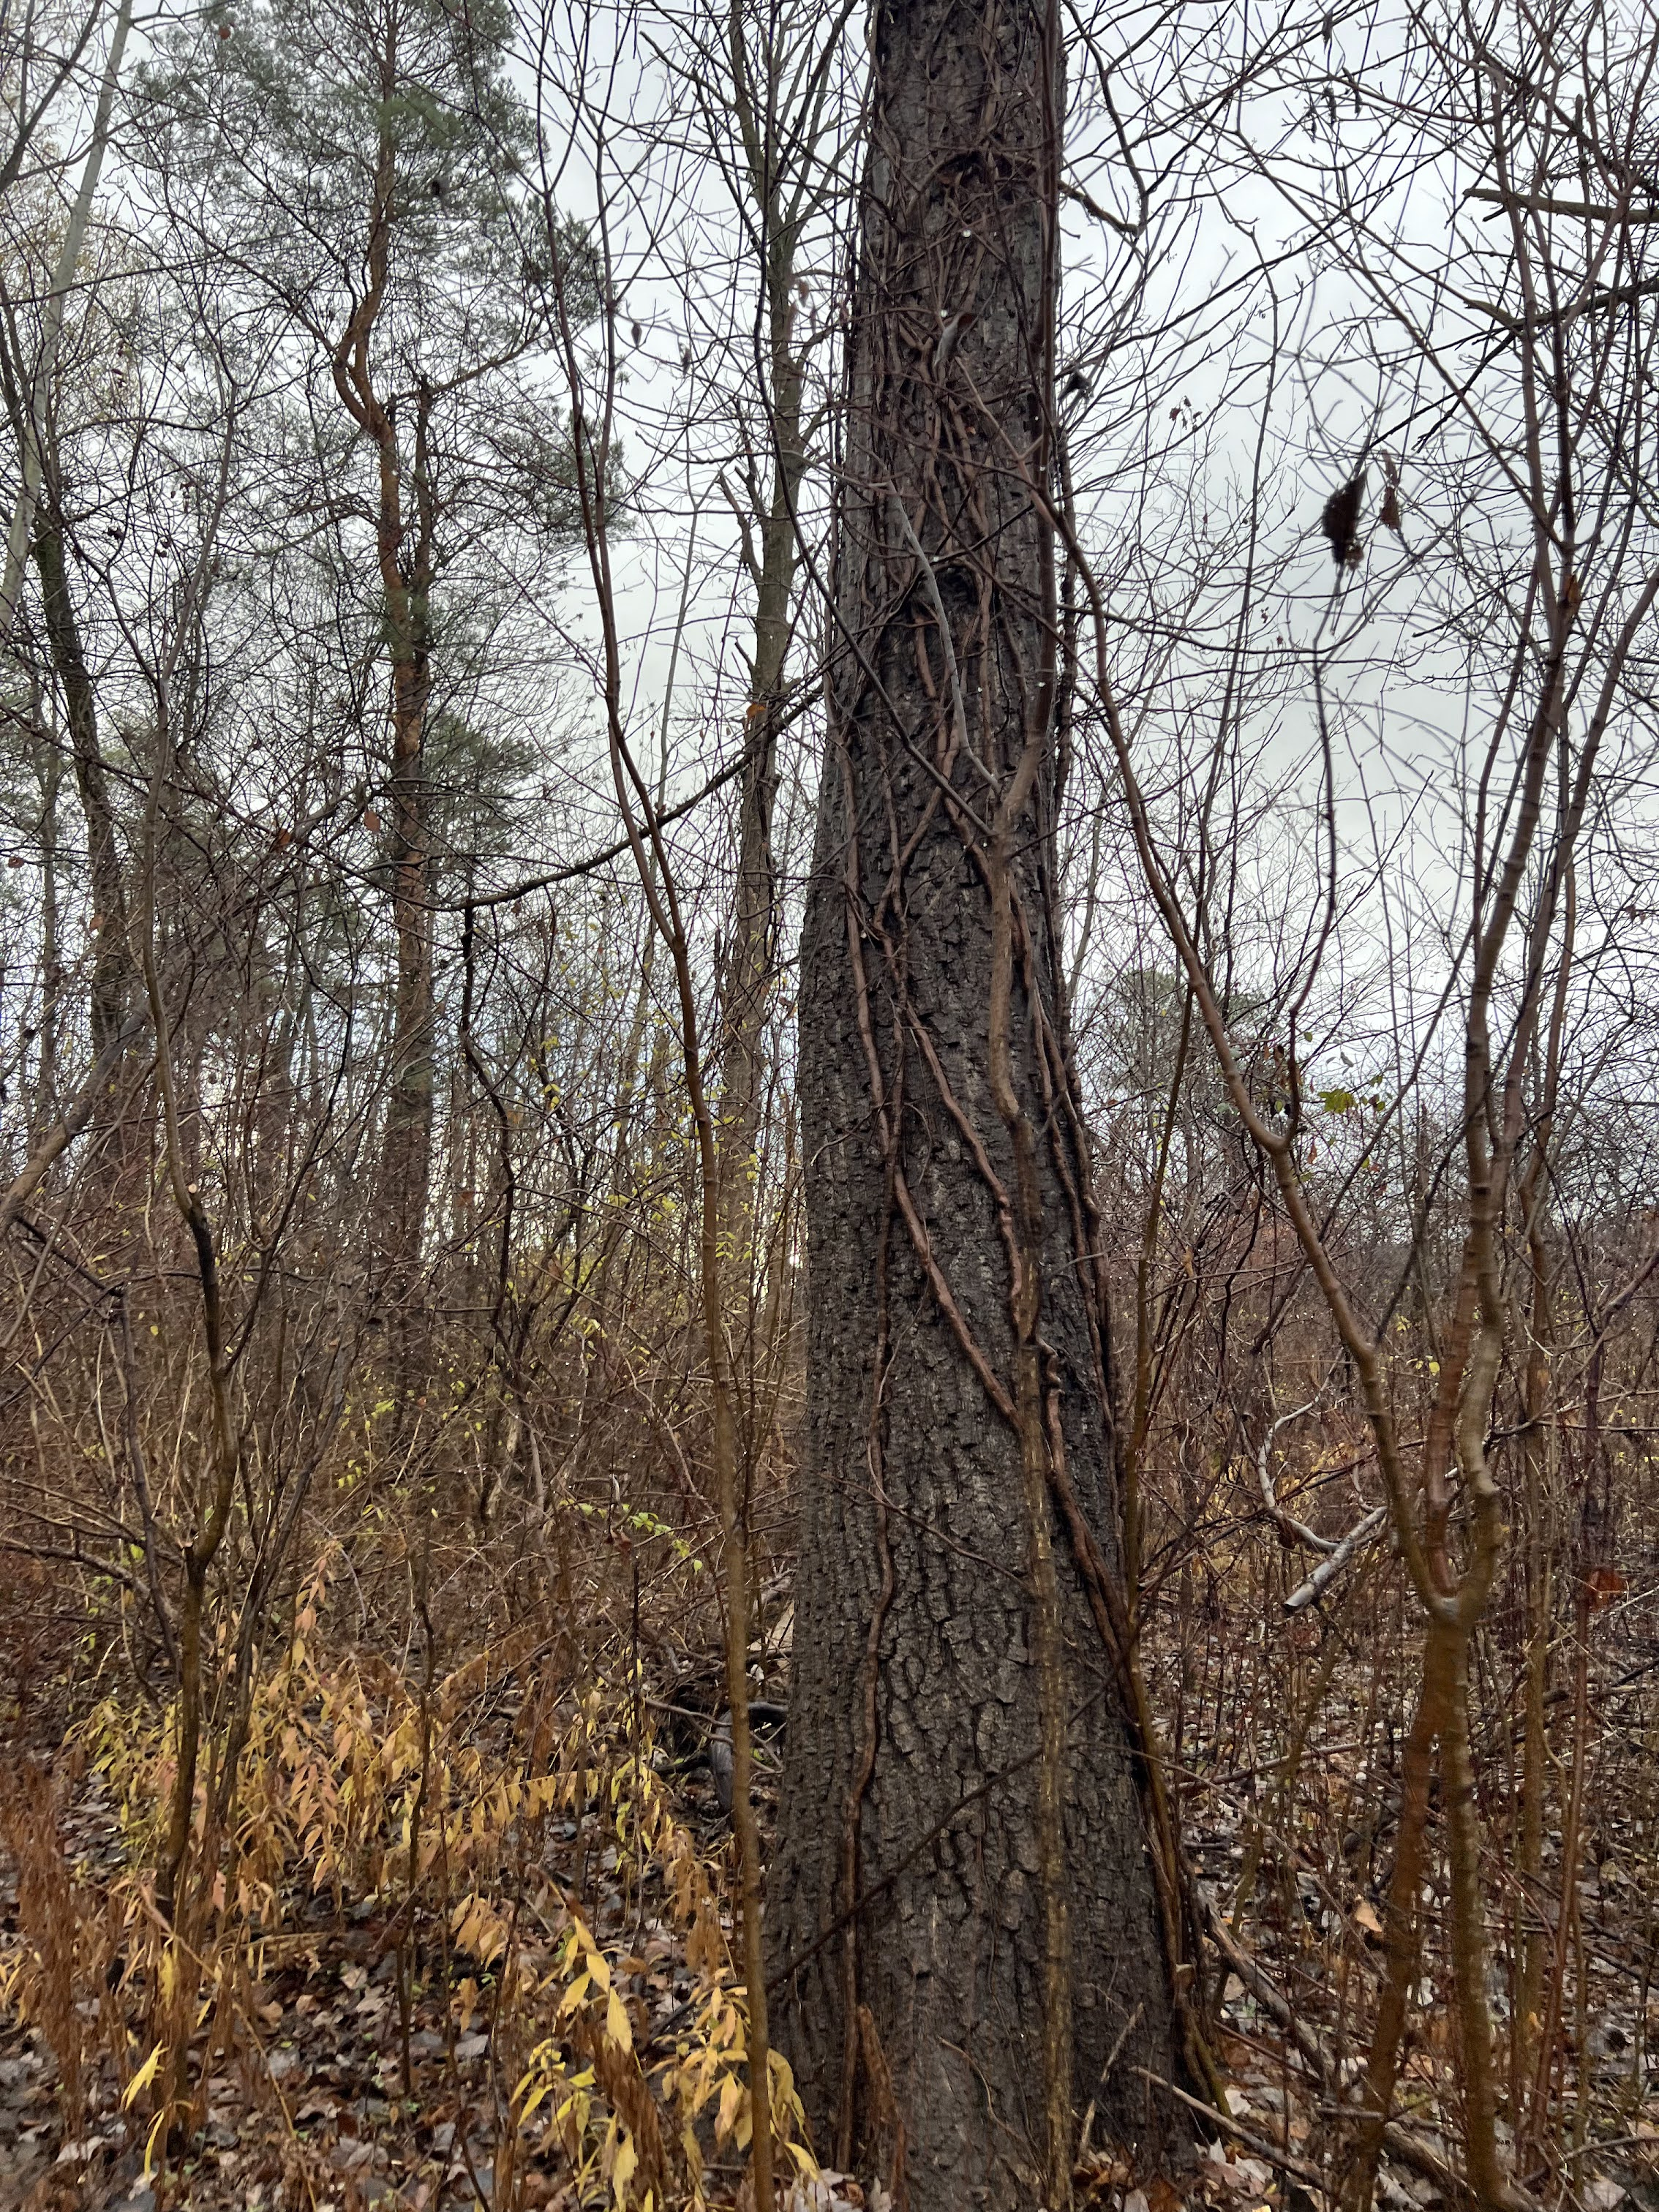
\includegraphics[scale=.1]{Research/HANA/NOV2024/IMG_9856.JPG}
\caption{HANA Tree Study}
\label{fig:HANA}
\end{figure}


\begin{figure}[h!]
\centering
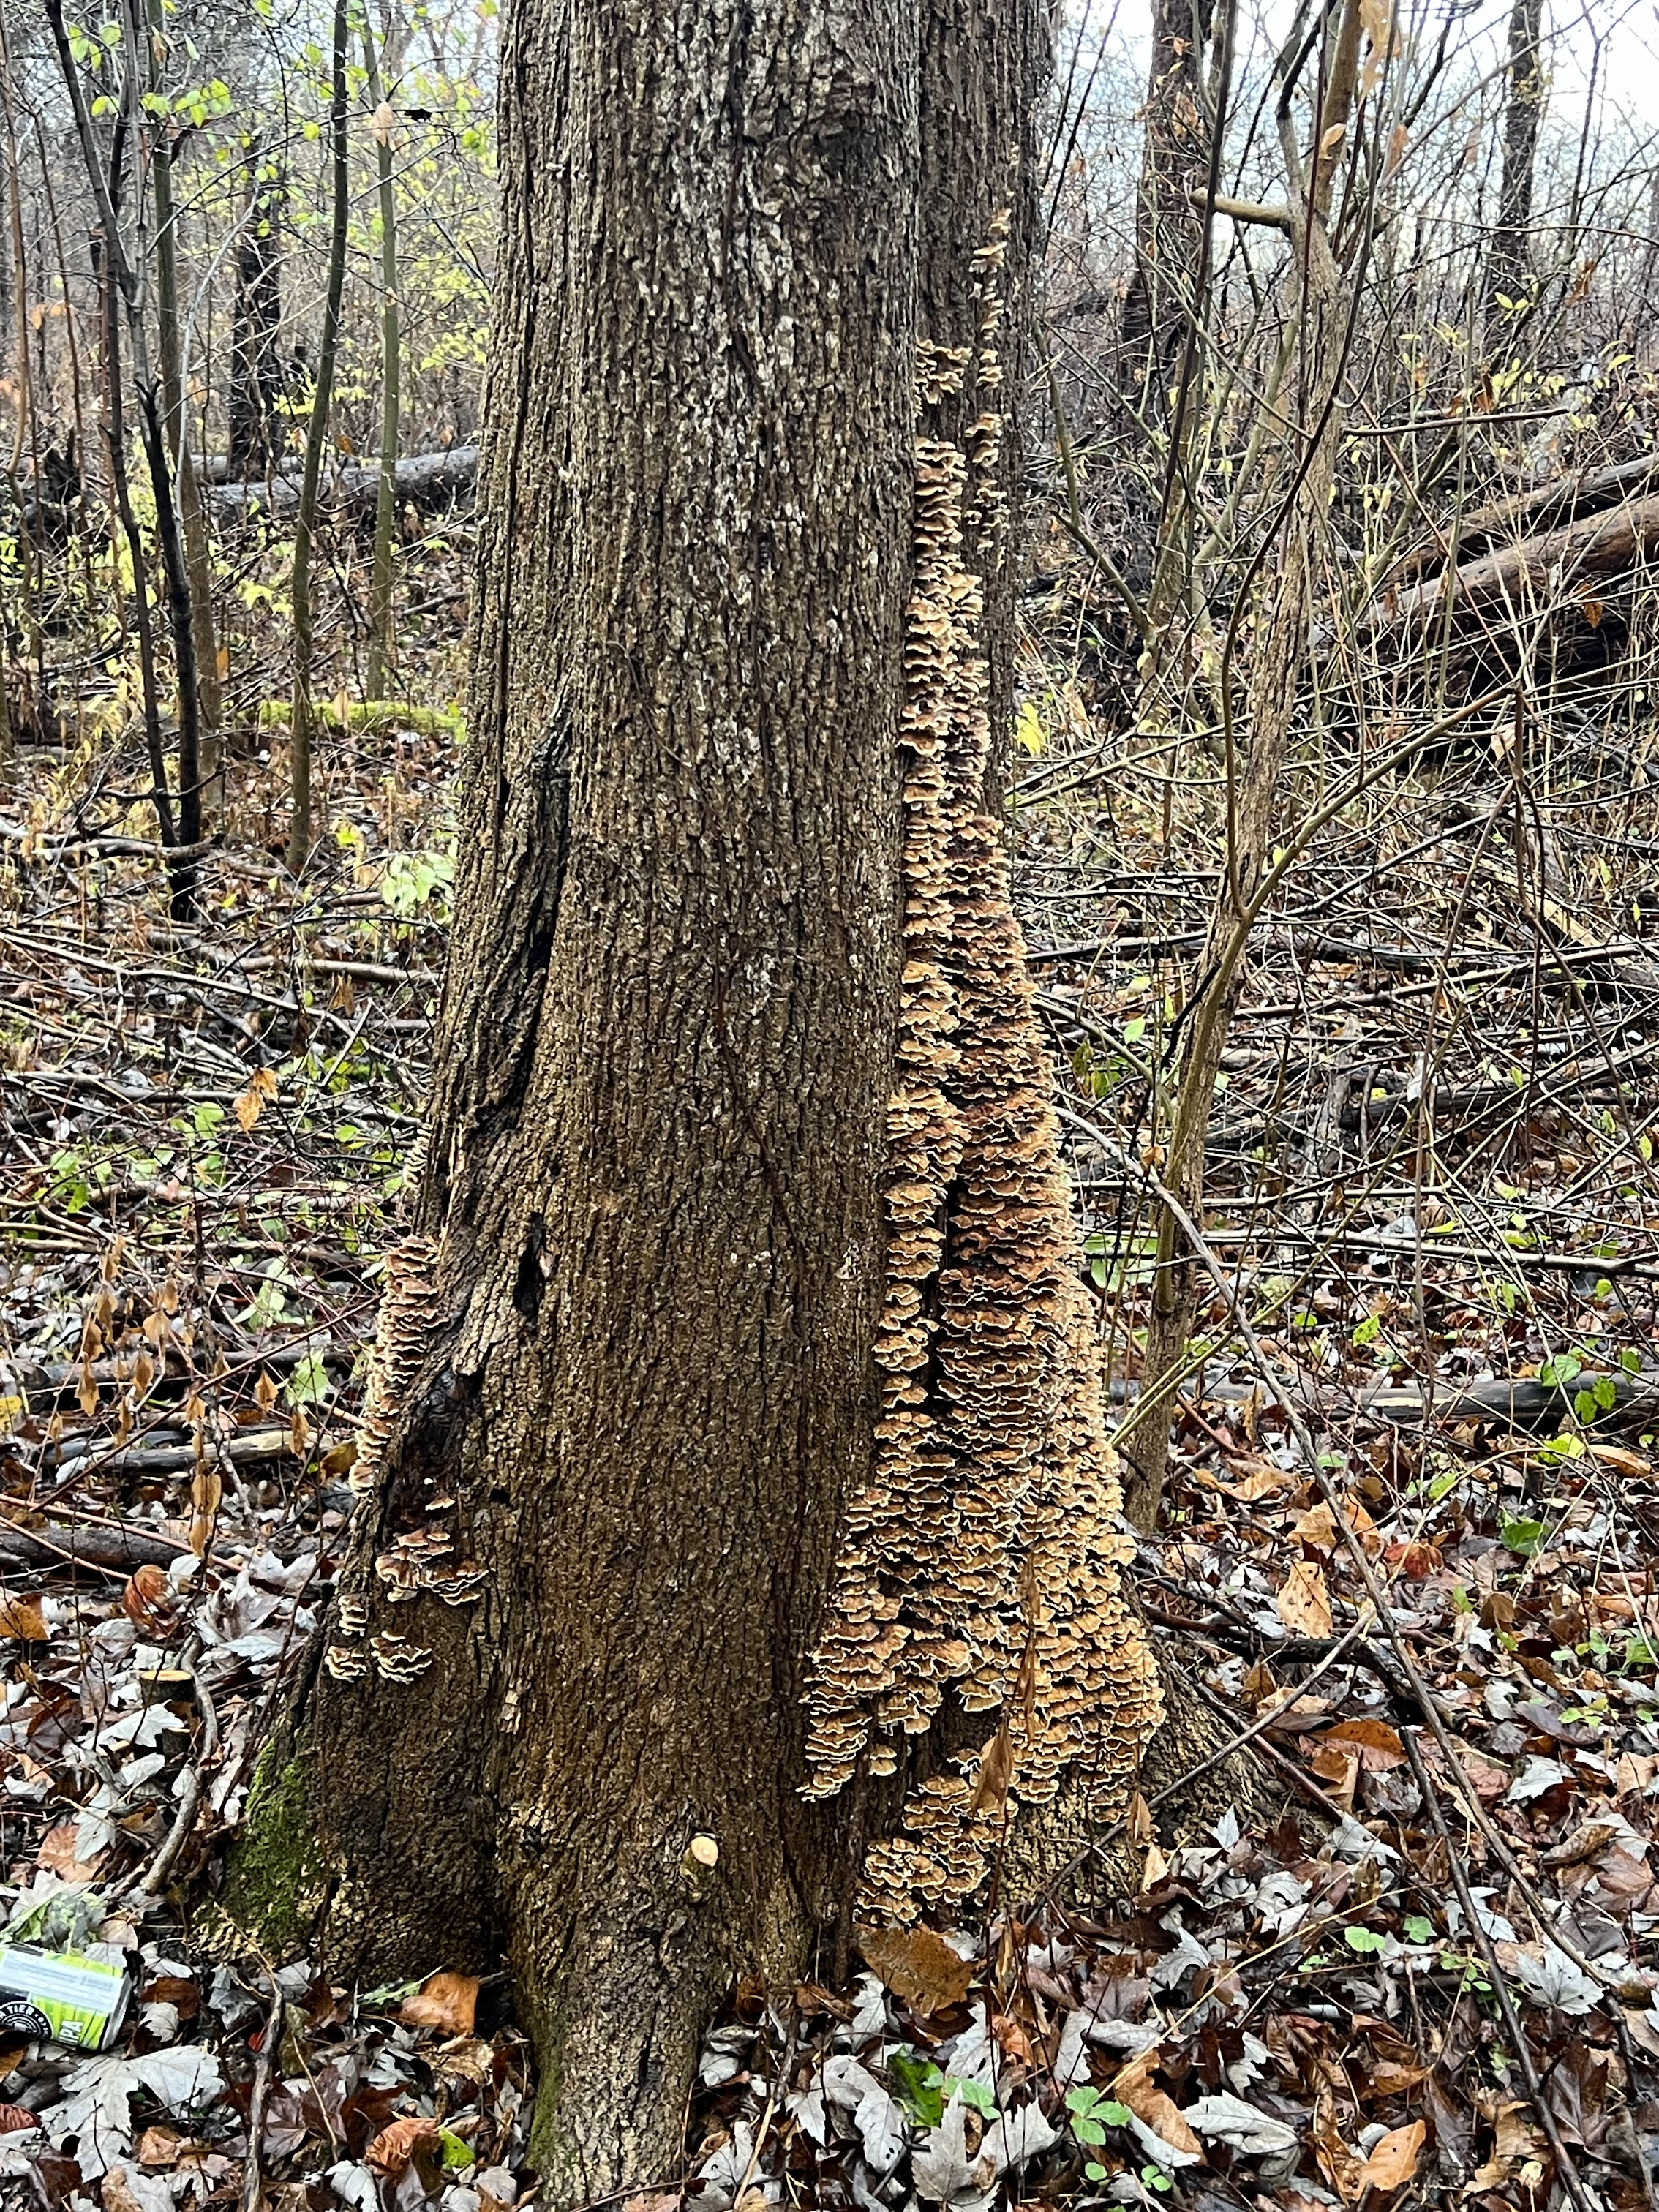
\includegraphics[scale=.1]{Research/HANA/NOV2024/IMG_9859.JPG}
\caption{HANA Tree Study}
\label{fig:HANA}
\end{figure}


\begin{figure}[h!]
\centering
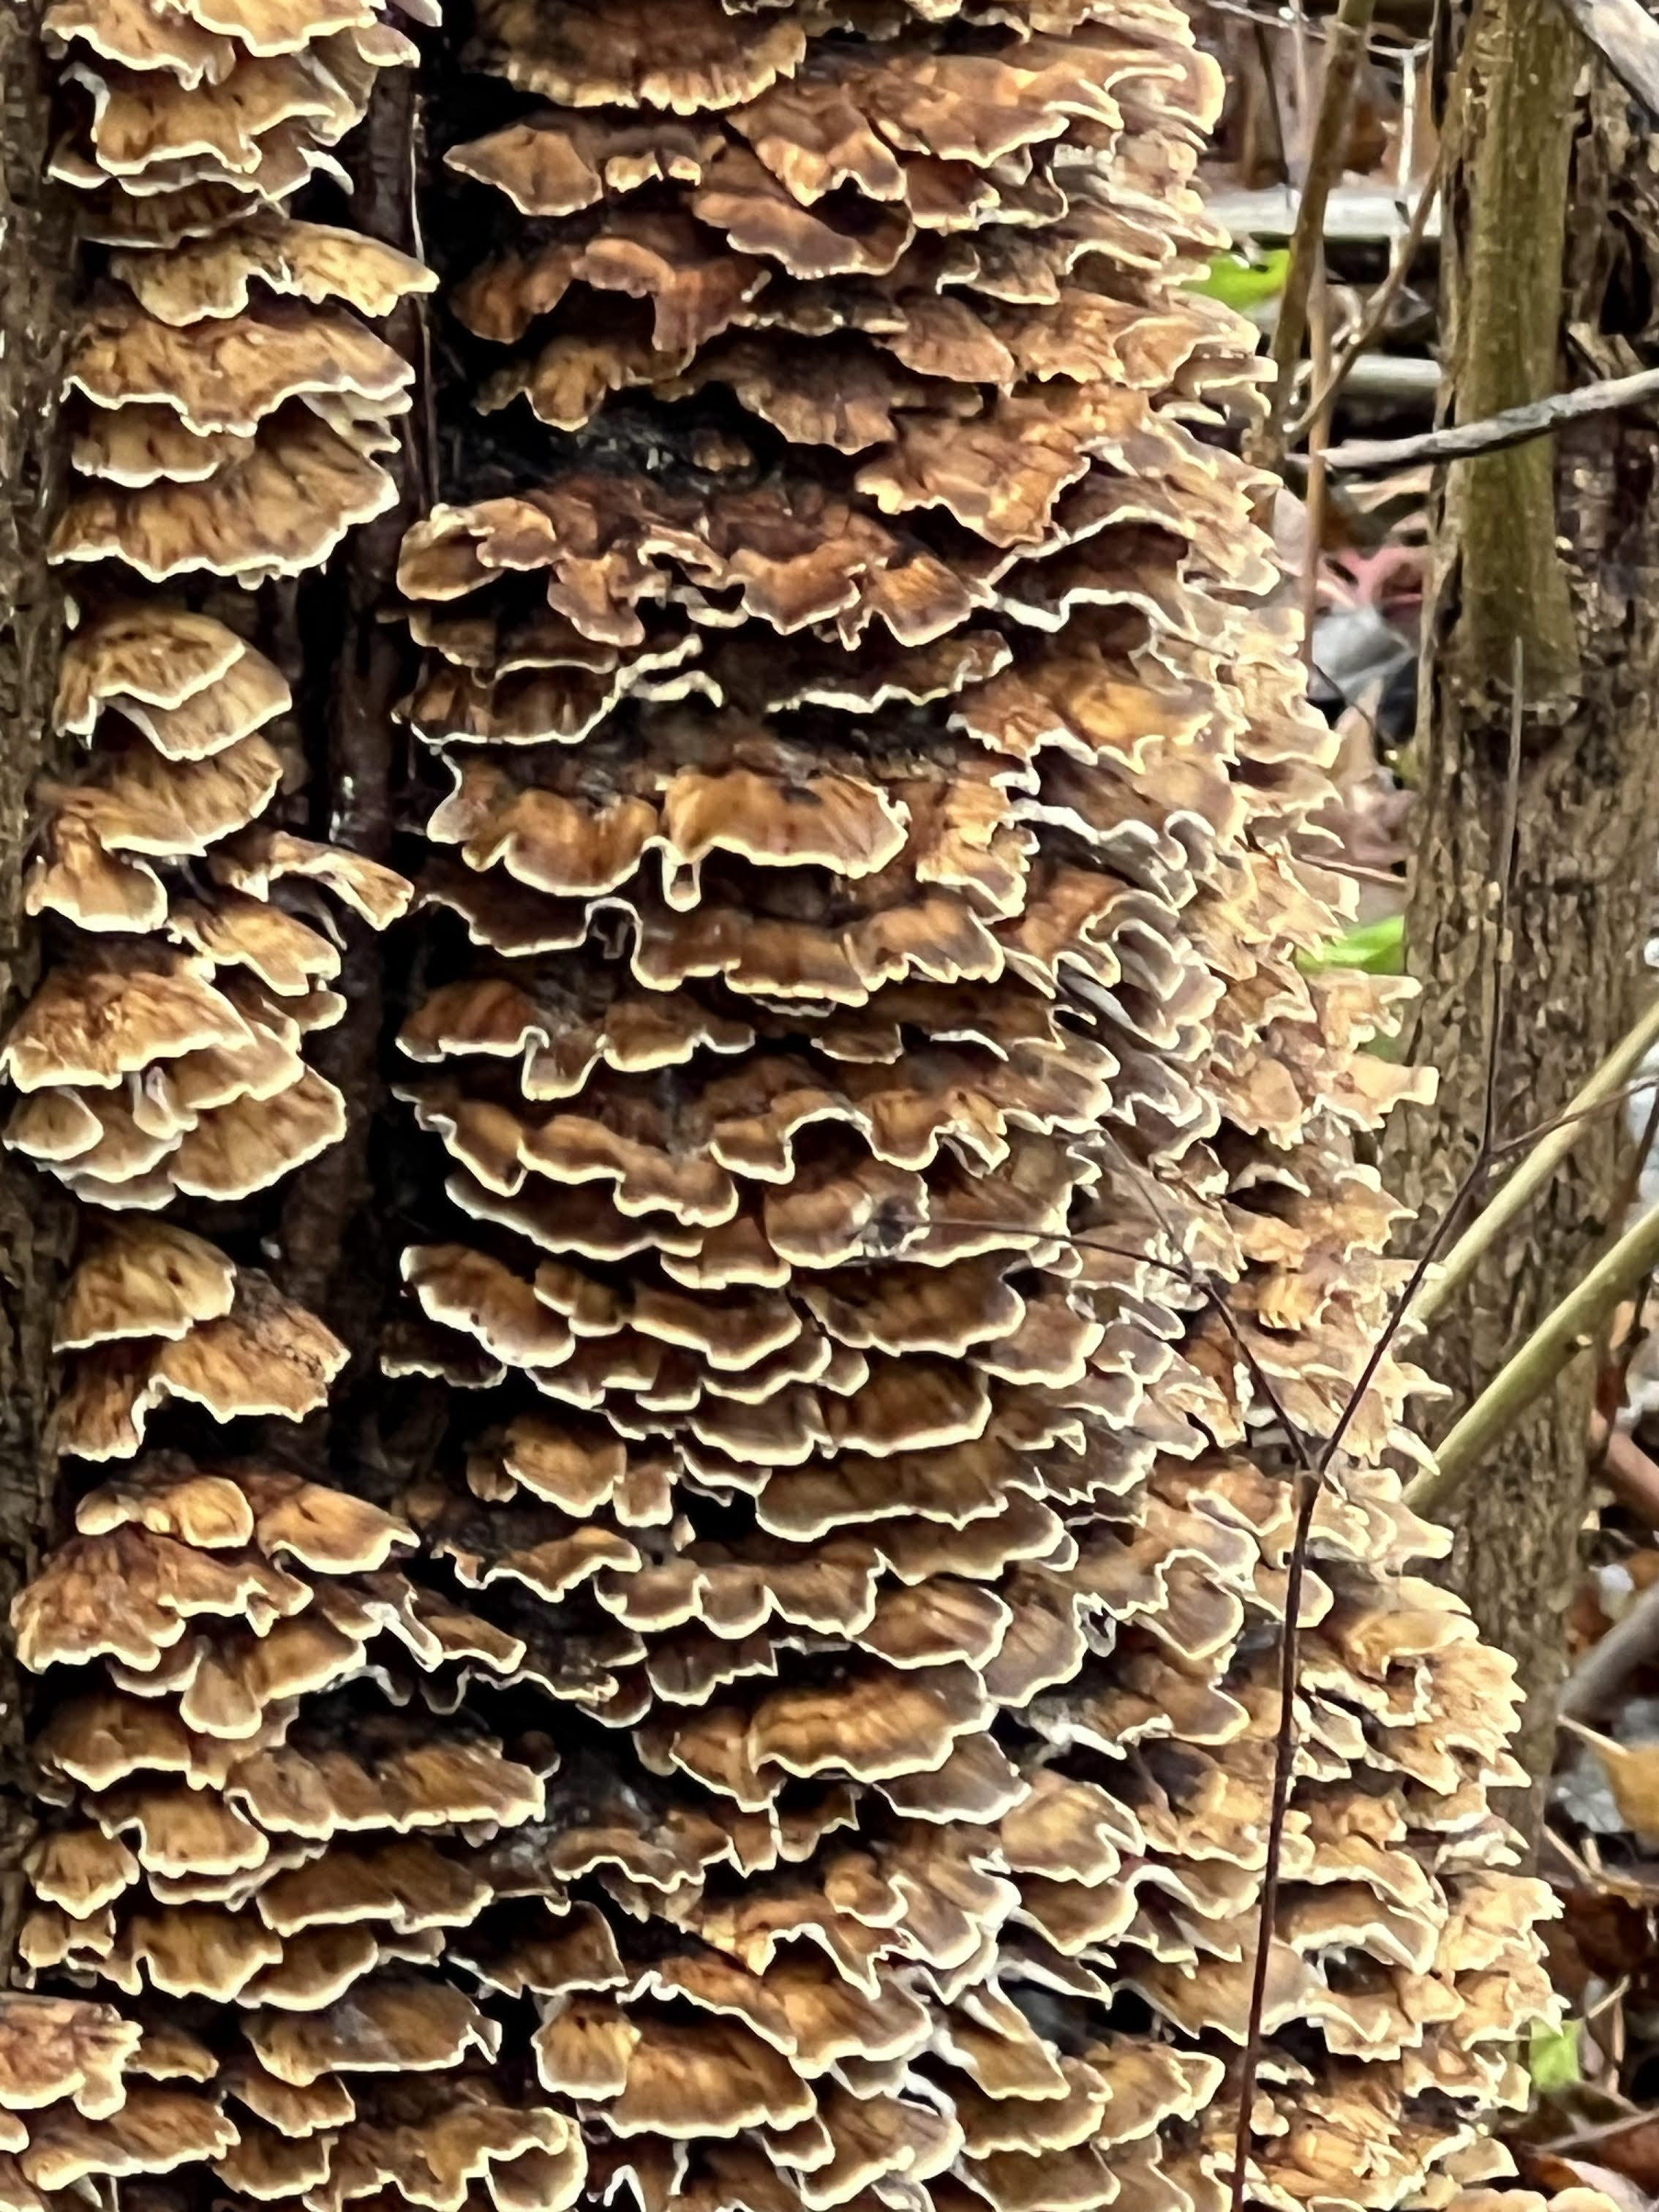
\includegraphics[scale=.1]{Research/HANA/NOV2024/IMG_9860.JPG}
\caption{HANA Tree Study}
\label{fig:HANA}
\end{figure}


\clearpage
\section{Bibliography}
\begin{thebibliography}{}

\bibitem{Calculus}
Stewart, James. Stewart Calculus. Cengage Learning Emea, 2014.

\bibitem{Fourier}
Easton, Roger Jr. Fourier Methods in Imaging. John Wiley and Sons, Incorporated, 2010.


\end{thebibliography}

\end{document}



